\documentclass[../main.tex]{subfiles}

\begin{document}

\chapter{Appendix}

\textbf{Versions}

\begin{table}[h]
\centering
\begin{minipage}{0.45\textwidth}
\centering
\begin{tabular}{|c|l|}
\hline
\textbf{Release Date} & \textbf{Product Version} \\ \hline
    2023-01-04 & Graylog 5.0.2 \\ \hline
    2023-01-04 & Graylog 4.3.11 \\ \hline  
    2023-02-01 & Graylog 4.3.12 \\ \hline  
    2023-02-01 & Graylog 5.0.3 \\ \hline  
    2023-03-01 & Graylog 5.0.4 \\ \hline  
    2023-03-01 & Graylog 4.3.13 \\ \hline  
    2023-03-06 & Graylog 5.0.5 \\ \hline  
    2023-04-05 & Graylog 4.3.14 \\ \hline  
    2023-04-05 & Graylog 5.0.6 \\ \hline  
    2023-05-03 & Graylog 4.3.15 \\ \hline  
    2023-05-03 & Graylog 5.0.7 \\ \hline  
    2023-05-11 & Graylog 5.1.0 \\ \hline  
    2023-05-25 & Graylog 5.1.1 \\ \hline  
    2023-06-07 & Graylog 5.0.8 \\ \hline  
    2023-06-07 & Graylog 5.1.2 \\ \hline  
    2023-07-05 & Graylog 5.0.9 \\ \hline  
    2023-07-05 & Graylog 5.1.3 \\ \hline  
    2023-08-02 & Graylog 5.0.10 \\ \hline  
    2023-08-02 & Graylog 5.1.4 \\ \hline  
    2023-09-06 & Graylog 5.0.11 \\ \hline  
    2023-08-02 & Graylog 5.1.5 \\ \hline  
    2023-10-04 & Graylog 5.0.12 \\ \hline  
    2023-10-04 & Graylog 5.1.6 \\ \hline  
    2023-10-12 & Graylog 5.1.7 \\ \hline  
    2023-10-12 & Graylog 5.0.13 \\ \hline  
    2023-11-01 & Graylog 5.2.0 \\ \hline  
    2023-11-01 & Graylog 5.1.8 \\ \hline  
    2023-11-15 & Graylog 5.2.1 \\ \hline  
    2023-12-06 & Graylog 5.1.9 \\ \hline  
    2023-12-06 & Graylog 5.2.2 \\ \hline  
\end{tabular}
\caption{Graylog Versions and Release Dates in Year 2023. Part 1}
\end{minipage}
\hspace{1cm} % Add space between tables
\begin{minipage}{0.45\textwidth}
\centering
\begin{tabular}{|c|l|}
\hline
\textbf{Release Date} & \textbf{Product Version} \\ \hline
    2024-01-03 & Graylog 5.1.10 \\ \hline  
    2024-01-03 & Graylog 5.2.3 \\ \hline  
    2024-02-07 & Graylog 5.1.11 \\ \hline  
    2024-02-07 & Graylog 5.2.4 \\ \hline  
    2024-03-06 & Graylog 5.1.12 \\ \hline  
    2024-03-06 & Graylog 5.2.5 \\ \hline  
    2024-04-03 & Graylog 5.1.13 \\ \hline  
    2024-04-03 & Graylog 5.2.6 \\ \hline  
    2024-04-30 & Graylog 5.2.7 \\ \hline  
    2024-04-17 & Graylog 6.0.0 \\ \hline  
    2024-05-13 & Graylog 6.0.1 \\ \hline  
    2024-05-22 & Graylog 6.0.2 \\ \hline  
    2024-06-05 & Graylog 6.0.3 \\ \hline  
    2024-06-05 & Graylog 5.2.8 \\ \hline  
    2024-07-03 & Graylog 5.2.9 \\ \hline  
    2024-07-03 & Graylog 6.0.4 \\ \hline  
    2024-08-07 & Graylog 5.2.10 \\ \hline  
    2024-08-07 & Graylog 6.0.5 \\ \hline  
    2024-09-04 & Graylog 5.2.11 \\ \hline  
    2024-09-04 & Graylog 6.0.6 \\ \hline  
    2024-10-02 & Graylog 5.2.12 \\ \hline  
    2024-10-02 & Graylog 6.0.7 \\ \hline  
    2024-10-12 & Graylog 6.1.0 \\ \hline  
    2024-10-23 & Graylog 6.1.1 \\ \hline  
    2024-11-06 & Graylog 6.0.8 \\ \hline  
    2024-11-06 & Graylog 6.1.2 \\ \hline  
    2024-11-21 & Graylog 6.1.3 \\ \hline  
    2024-12-04 & Graylog 6.0.9 \\ \hline  
    2024-12-04 & Graylog 6.1.4 \\ \hline  
\end{tabular}
\caption{Graylog Versions and Release Dates in Year 2024. Part 2 https://graylog.org/releases/}
\label{table:graylog_versions}
\end{minipage}
\end{table}


\begin{table}[h]
\centering
\begin{minipage}{0.45\textwidth}
\centering
\begin{tabular}{|c|l|}
\hline
\textbf{Product Version} & \textbf{Release Date} \\ \hline
    2023-02-27 & MongoDB 5.0.15 \\ \hline
    2023-04-10 & MongoDB 5.0.16 \\ \hline
    2023-04-27 & MongoDB 5.0.17 \\ \hline
    2023-05-18 & MongoDB 5.0.18 \\ \hline
    2023-07-13 & MongoDB 5.0.19 \\ \hline
    2023-08-14 & MongoDB 5.0.20 \\ \hline
    2023-09-12 & MongoDB 5.0.21 \\ \hline
    2023-10-26 & MongoDB 5.0.22 \\ \hline
    2023-11-27 & MongoDB 5.0.23 \\ \hline
    2024-01-18 & MongoDB 5.0.24 \\ \hline
    2024-02-28 & MongoDB 5.0.25 \\ \hline
    2024-03-26 & MongoDB 5.0.26 \\ \hline
    2024-06-04 & MongoDB 5.0.27 \\ \hline
    2024-07-15 & MongoDB 5.0.28 \\ \hline
    2024-09-30 & MongoDB 5.0.29 \\ \hline
    2024-10-24 & MongoDB 5.0.30 \\ \hline
\end{tabular}
\caption{MongoDB 5.x Versions and Release Dates. https://www.mongodb.com/docs/upcoming/release-notes/5.0/}
\end{minipage}
\hspace{1cm} % Add space between tables
\begin{minipage}{0.45\textwidth}
\centering
\begin{tabular}{|c|l|}
\hline
\textbf{Release Date} & \textbf{Product Version} \\ \hline
    2023-01-26 & MongoDB 6.0.4 \\ \hline
    2023-03-13 & MongoDB 6.0.5 \\ \hline
    2023-05-12 & MongoDB 6.0.6 \\ \hline
    2023-06-28 & MongoDB 6.0.7 \\ \hline
    2023-07-13 & MongoDB 6.0.8 \\ \hline
    2023-08-14 & MongoDB 6.0.9 \\ \hline
    2023-09-14 & MongoDB 6.0.10 \\ \hline
    2023-10-11 & MongoDB 6.0.11 \\ \hline
    2023-11-27 & MongoDB 6.0.12 \\ \hline
    2024-01-18 & MongoDB 6.0.13 \\ \hline
    2024-02-28 & MongoDB 6.0.14 \\ \hline
    2024-04-18 & MongoDB 6.0.15 \\ \hline
    2024-06-28 & MongoDB 6.0.16 \\ \hline
    2024-08-21 & MongoDB 6.0.17 \\ \hline
    2024-09-30 & MongoDB 6.0.18 \\ \hline
    2024-10-24 & MongoDB 6.0.19 \\ \hline
\end{tabular}
\caption{MongoDB 6.x Versions and Release Dates. https://www.mongodb.com/docs/upcoming/release-notes/6.0/}
\label{table:mongodb_versions}
\end{minipage}
\end{table}

\begin{table}[h]
\centering
\begin{tabular}{|c|l|}
\hline
\textbf{Release Date} & \textbf{Product Version} \\ \hline
    2023-08-15 & MongoDB 7.0.0 \\ \hline
    2023-09-05 & MongoDB 7.0.1 \\ \hline
    2023-09-29 & MongoDB 7.0.2 \\ \hline
    2023-11-09 & MongoDB 7.0.3 \\ \hline
    2023-11-27 & MongoDB 7.0.4 \\ \hline
    2024-01-05 & MongoDB 7.0.5 \\ \hline
    2024-02-28 & MongoDB 7.0.6 \\ \hline
    2024-03-18 & MongoDB 7.0.7 \\ \hline
    2024-04-03 & MongoDB 7.0.8 \\ \hline
    2024-04-26 & MongoDB 7.0.9 \\ \hline
    2024-05-23 & MongoDB 7.0.11 \\ \hline
    2024-06-28 & MongoDB 7.0.12 \\ \hline
    2024-08-26 & MongoDB 7.0.14 \\ \hline
    2024-10-24 & MongoDB 7.0.15 \\ \hline
    2024-12-20 & MongoDB 7.0.16 \\ \hline
\end{tabular}
\caption{MongoDB 7.x Versions and Release Dates. https://www.mongodb.com/docs/upcoming/release-notes/7.0/}
\label{table:mongodb_versions}
\end{table}

\begin{table}[h]
\centering
\begin{tabular}{|c|l|}
\hline
\textbf{Release Date} & \textbf{Product Version} \\ \hline
    2023-01-24 & OpenSearch 2.5.0 \\ \hline  
    2023-02-02 & OpenSearch 1.3.8 \\ \hline  
    2023-02-28 & OpenSearch 2.6.0 \\ \hline  
    2023-03-16 & OpenSearch 1.3.9 \\ \hline  
    2023-05-02 & OpenSearch 2.7.0 \\ \hline  
    2023-05-18 & OpenSearch 1.3.10 \\ \hline  
    2023-06-06 & OpenSearch 2.8.0 \\ \hline  
    2023-06-29 & OpenSearch 1.3.11 \\ \hline  
    2023-07-24 & OpenSearch 2.9.0 \\ \hline  
    2023-08-10 & OpenSearch 1.3.12 \\ \hline  
    2023-09-21 & OpenSearch 1.3.13 \\ \hline  
    2023-09-25 & OpenSearch 2.10.0 \\ \hline  
    2023-10-16 & OpenSearch 2.11.0 \\ \hline  
    2023-11-30 & OpenSearch 2.11.1 \\ \hline  
    2023-12-12 & OpenSearch 1.3.14 \\ \hline  
    2024-02-20 & OpenSearch 2.12.0 \\ \hline  
    2024-04-02 & OpenSearch 2.13.0 \\ \hline  
    2024-05-14 & OpenSearch 2.14.0 \\ \hline  
    2024-06-25 & OpenSearch 2.15.0 \\ \hline  
    2024-08-06 & OpenSearch 2.16.0 \\ \hline  
    2024-09-17 & OpenSearch 2.17.0 \\ \hline  
    2024-10-01 & OpenSearch 2.17.1 \\ \hline  
    2024-11-05 & OpenSearch 2.18.0 \\ \hline
\end{tabular}
\caption{OpenSearch Versions and Release Dates https://opensearch.org/docs/latest/version-history/}
\label{table:opensearch_versions}
\end{table}

\begin{table}[h]
    \centering
    \begin{tabular}{|c|c|}
        \hline
        \textbf{Release Date} & \textbf{Product Version} \\
        \hline
        2023-03-04 & Logging Operator 4.0.0 \\
        2023-04-12 & Logging Operator 4.1.0 \\
        2023-05-23 & Logging Operator 3.17.11 \\
        2023-06-05 & Logging Operator 4.2.0 \\
        2023-06-08 & Logging Operator 4.2.1 \\
        2023-06-13 & Logging Operator 4.2.2 \\
        2023-08-10 & Logging Operator 4.3.0 \\
        2023-09-29 & Logging Operator 4.4.0 \\
        2023-10-20 & Logging Operator 4.4.1 \\
        2023-11-14 & Logging Operator 4.4.2 \\
        2023-11-24 & Logging Operator 4.4.3 \\
        2023-12-12 & Logging Operator 4.5.0 \\
        2024-01-11 & Logging Operator 4.5.1 \\
        2024-01-25 & Logging Operator 4.5.2 \\
        2024-01-29 & Logging Operator 4.5.3 \\
        2024-02-06 & Logging Operator 4.5.4 \\
        2024-02-07 & Logging Operator 4.5.5 \\
        2024-02-09 & Logging Operator 4.5.6 \\
        2024-03-18 & Logging Operator 4.6.0 \\
        2024-05-22 & Logging Operator 4.6.1 \\
        2024-06-03 & Logging Operator 4.7.0 \\
        2024-06-06 & Logging Operator 4.6.2 \\
        2024-07-02 & Logging Operator 4.8.0 \\
        2024-08-13 & Logging Operator 4.9.0 \\
        2024-08-27 & Logging Operator 4.9.1 \\
        2024-10-03 & Logging Operator 4.10.0 \\
        2024-11-08 & Logging Operator 4.10.1 \\
        2024-11-13 & Logging Operator 4.11.0 \\
        2024-12-11 & Logging Operator 4.11.2 \\
        2024-12-16 & Logging Operator 4.10.2 \\
        2024-12-16 & Logging Operator 4.10.3 \\
        2024-12-17 & Logging Operator 4.10.4 \\
        2024-12-17 & Logging Operator 4.11.3 \\
        2024-12-17 & Logging Operator 5.0.0 \\
        2024-12-19 & Logging Operator 4.11.4 \\
        2024-12-19 & Logging Operator 5.0.1 \\
        \hline
    \end{tabular}
   \caption{Logging Operator versions and release dates (excluding pre-releases). Source: https://github.com/kube-logging/logging-operator/releases}
   \label{tab:logging_operator_versions}
\end{table}

\begin{table}[h]
\centering
\begin{minipage}{0.45\textwidth}
\centering
\begin{tabular}{|c|l|}
\hline
\textbf{Release Date} & \textbf{Helm Chart Version} \\ \hline
    2023-01-14 & MongoDB 13.6.3(6.0.3) \\ \hline
    2023-01-19 & MongoDB 13.6.4(6.0.4) \\ \hline  
    2023-01-25 & MongoDB 13.6.5(6.0.4) \\ \hline
    2023-01-25 & MongoDB 13.6.6(6.0.4) \\ \hline 
    2023-01-31 & MongoDB 13.6.7(6.0.4) \\ \hline 
    2023-02-20 & MongoDB 13.6.8(6.0.4) \\ \hline
    2023-02-21 & MongoDB 13.7.0(6.0.4) \\ \hline
    2023-02-22 & MongoDB 13.8.0(6.0.4) \\ \hline
    2023-02-22 & MongoDB 13.8.1(6.0.4) \\ \hline
    2023-03-01 & MongoDB 13.8.2(6.0.4) \\ \hline 
    2023-03-08 & MongoDB 13.8.3(6.0.4) \\ \hline 
    2023-03-10 & MongoDB 13.9.0(6.0.4) \\ \hline 
    2023-03-14 & MongoDB 13.9.1(6.0.5) \\ \hline  
    2023-03-20 & MongoDB 13.9.2(6.0.5)\\ \hline  
    2023-03-24 & MongoDB 13.9.3(6.0.5) \\ \hline
    2023-04-01 & MongoDB 13.9.4(6.0.5) \\ \hline  
    2023-04-27 & MongoDB 13.10.1(6.0.5) \\ \hline
    2023-05-01 & MongoDB 13.10.2(6.0.5) \\ \hline
    2023-05-09 & MongoDB 13.10.3(6.0.5) \\ \hline
    2023-05-12 & MongoDB 13.12.0(6.0.5) \\ \hline
    2023-05-12 & MongoDB 13.12.1(6.0.6) \\ \hline  
    2023-05-17 & MongoDB 13.13.0(6.0.6) \\ \hline  
    2023-05-21 & MongoDB 13.13.1(6.0.6) \\ \hline  
    2023-05-22 & MongoDB 13.14.0(6.0.6) \\ \hline 
    2023-05-22 & MongoDB 13.14.1(6.0.6) \\ \hline  
    2023-05-24 & MongoDB 13.14.2(6.0.6) \\ \hline  
    2023-05-24 & MongoDB 13.15.0(6.0.6) \\ \hline  
    2023-05-25 & MongoDB 13.15.1(6.0.6) \\ \hline 
    2023-06-19 & MongoDB 13.15.2(6.0.6) \\ \hline 
    2023-06-20 & MongoDB 13.15.3(6.0.6) \\ \hline 
    2023-07-01 & MongoDB 13.15.4(6.0.7) \\ \hline 
    2023-07-15 & MongoDB 13.15.5(6.0.8) \\ \hline  
    2023-07-18 & MongoDB 13.16.0(6.0.8) \\ \hline 
    2023-07-26 & MongoDB 13.16.1(6.0.8) \\ \hline  
    2023-07-31 & MongoDB 13.16.2(6.0.8) \\ \hline
    2023-08-09 & MongoDB 13.16.3(6.0.8) \\ \hline
    2023-08-17 & MongoDB 13.16.4(6.0.8) \\ \hline  
    2023-08-23 & MongoDB 13.17.0(6.0.8) \\ \hline
    2023-08-25 & MongoDB 13.17.1(6.0.9) \\ \hline
    2023-08-28 & MongoDB 13.17.2(6.0.9) \\ \hline 
    2023-08-30 & MongoDB 13.18.0(6.0.9) \\ \hline  
    2023-08-30 & MongoDB 13.18.1(6.0.9) \\ \hline
\end{tabular}
\caption{MongoDB Helm Chart Versions and Release Dates in Year 2023. Part 1 https://artifacthub.io/packages/helm/bitnami/mongodb}
\end{minipage}
\hspace{1cm} % Add space between tables
\begin{minipage}{0.45\textwidth}
\centering
\begin{tabular}{|c|l|}
\hline
\textbf{Release Date} & \textbf{Helm Chart Version} \\ \hline
    2023-09-11 & MongoDB 13.18.2(6.0.9) \\ \hline
    2023-09-14 & MongoDB 13.18.3(6.0.10) \\ \hline  
    2023-09-15 & MongoDB 13.18.4(6.0.10) \\ \hline  
    2023-09-22 & MongoDB 13.18.5(6.0.10) \\ \hline  
    2023-09-22 & MongoDB 14.0.0(7.0.1) \\ \hline  
    2023-09-25 & MongoDB 14.0.1(7.0.1) \\ \hline  
    2023-09-27 & MongoDB 14.0.2(7.0.1) \\ \hline  
    2023-09-29 & MongoDB 14.0.3(7.0.1) \\ \hline  
    2023-09-30 & MongoDB 14.0.4(7.0.2) \\ \hline  
    2023-10-05 & MongoDB 14.0.5(7.0.2) \\ \hline   
    2023-10-09 & MongoDB 14.0.6(7.0.2) \\ \hline   
    2023-10-09 & MongoDB 14.0.7(7.0.2) \\ \hline   
    2023-10-10 & MongoDB 14.0.9(7.0.2) \\ \hline  
    2023-10-12 & MongoDB 14.0.10(7.0.2) \\ \hline  
    2023-10-19 & MongoDB 14.0.11(7.0.2) \\ \hline 
    2023-10-21 & MongoDB 14.0.12(7.0.2) \\ \hline  
    2023-10-25 & MongoDB 14.0.13(7.0.2) \\ \hline  
    2023-10-27 & MongoDB 14.0.14(7.0.2) \\ \hline 
    2023-10-31 & MongoDB 14.1.0(7.0.2) \\ \hline 
    2023-11-06 & MongoDB 14.1.1(7.0.2) \\ \hline  
    2023-11-07 & MongoDB 14.2.0(7.0.2) \\ \hline  
    2023-11-08 & MongoDB 14.2.1(7.0.2) \\ \hline  
    2023-11-09 & MongoDB 14.2.2(7.0.2) \\ \hline  
    2023-11-09 & MongoDB 14.2.3(7.0.3) \\ \hline  
    2023-11-10 & MongoDB 14.2.4(7.0.3) \\ \hline  
    2023-11-10 & MongoDB 14.2.5(7.0.3) \\ \hline  
    2023-11-14 & MongoDB 14.2.6(7.0.3) \\ \hline  
    2023-11-17 & MongoDB 14.2.7(7.0.3) \\ \hline  
    2023-11-17 & MongoDB 14.2.8(7.0.3) \\ \hline  
    2023-11-20 & MongoDB 14.3.0(7.0.3) \\ \hline  
    2023-11-22 & MongoDB 14.3.1(7.0.3) \\ \hline  
    2023-11-27 & MongoDB 14.3.2(7.0.4) \\ \hline
    2023-12-04 & MongoDB 14.4.0(7.0.4) \\ \hline  
    2023-12-05 & MongoDB 14.4.1(7.0.4) \\ \hline  
    2023-12-07 & MongoDB 14.4.2(7.0.4) \\ \hline  
    2023-12-18 & MongoDB 14.4.3(7.0.4) \\ \hline  
    2023-12-21 & MongoDB 14.4.4(7.0.4) \\ \hline  
    2023-12-21 & MongoDB 14.4.5(7.0.4) \\ \hline  
    2023-12-22 & MongoDB 14.4.6(7.0.4) \\ \hline  
    2023-12-26 & MongoDB 14.4.7(7.0.4) \\ \hline  
    2023-12-27 & MongoDB 14.4.8(7.0.4) \\ \hline  
    2023-12-29 & MongoDB 14.4.9(7.0.4) \\ \hline
\end{tabular}
\caption{MongoDB Helm Chart Versions and Release Dates in Year 2023. Part 2 https://artifacthub.io/packages/helm/bitnami/mongodb}
\label{table:mongodb_helm_versions}
\end{minipage}
\end{table}


\begin{table}[h]
\centering
\begin{minipage}{0.45\textwidth}
\centering
\begin{tabular}{|c|l|}
\hline
\textbf{Release Date} & \textbf{Helm Chart Version} \\ \hline
    2024-01-06 & MongoDB 14.4.10(7.0.5) \\ \hline   
    2024-01-08 & MongoDB 14.5.0(7.0.5) \\ \hline   
    2024-01-15 & MongoDB 14.5.1(7.0.5) \\ \hline  
    2024-01-17 & MongoDB 14.6.0(7.0.5) \\ \hline  
    2024-01-18 & MongoDB 14.6.1(7.0.5) \\ \hline  
    2024-01-22 & MongoDB 14.7.0(7.0.5) \\ \hline  
    2024-01-29 & MongoDB 14.7.2(7.0.5) \\ \hline  
    2024-01-31 & MongoDB 14.7.3(7.0.5) \\ \hline
    2024-02-01 & MongoDB 14.8.0(7.0.5) \\ \hline  
    2024-02-02 & MongoDB 14.8.1(7.0.5) \\ \hline  
    2024-02-03 & MongoDB 14.8.2(7.0.5) \\ \hline  
    2024-02-05 & MongoDB 14.8.3(7.0.5) \\ \hline  
    2024-02-15 & MongoDB 14.9.0(7.0.5) \\ \hline  
    2024-02-16 & MongoDB 14.10.0(7.0.5) \\ \hline
    2024-02-19 & MongoDB 14.10.1(7.0.5) \\ \hline  
    2024-02-21 & MongoDB 14.11.1(7.0.5) \\ \hline  
    2024-02-22 & MongoDB 14.12.0(7.0.5) \\ \hline  
    2024-02-22 & MongoDB 14.12.1(7.0.5) \\ \hline  
    2024-02-27 & MongoDB 14.12.2(7.0.5) \\ \hline  
    2024-02-29 & MongoDB 14.12.3(7.0.6) \\ \hline  
    2024-03-06 & MongoDB 14.13.0(7.0.6) \\ \hline
    2024-03-18 & MongoDB 15.0.0(7.0.6) \\ \hline  
    2024-03-18 & MongoDB 15.0.1(7.0.7) \\ \hline
    2024-03-19 & MongoDB 15.0.2(7.0.7) \\ \hline 
    2024-03-21 & MongoDB 15.1.0(7.0.7) \\ \hline 
    2024-04-01 & MongoDB 15.1.1(7.0.7) \\ \hline  
    2024-04-04 & MongoDB 15.1.2(7.0.8) \\ \hline  
    2024-04-05 & MongoDB 15.1.3(7.0.8) \\ \hline  
    2024-04-09 & MongoDB 15.1.4(7.0.8) \\ \hline  
    2024-04-23 & MongoDB 15.1.5(7.0.8) \\ \hline  
    2024-04-26 & MongoDB 15.1.6(7.0.8) \\ \hline  
    2024-04-27 & MongoDB 15.1.7(7.0.9) \\ \hline
    2024-05-09 & MongoDB 15.2.0(7.0.9) \\ \hline  
    2024-05-10 & MongoDB 15.3.0(7.0.9) \\ \hline  
    2024-05-13 & MongoDB 15.3.1(7.0.9) \\ \hline  
    2024-05-13 & MongoDB 15.4.0(7.0.9) \\ \hline
\end{tabular}
\caption{MongoDB Helm Chart Versions and Release Dates in Year 2024. Part 1 https://artifacthub.io/packages/helm/bitnami/mongodb}
\end{minipage}
\hspace{1cm} % Add space between tables
\begin{minipage}{0.45\textwidth}
\centering
\begin{tabular}{|c|l|}
\hline
\textbf{Release Date} & \textbf{Helm Chart Version} \\ \hline
    2024-05-13 & MongoDB 15.4.1(7.0.9) \\ \hline
    2024-05-14 & MongoDB 15.4.2(7.0.9) \\ \hline
    2024-05-14 & MongoDB 15.4.3(7.0.9) \\ \hline
    2024-05-18 & MongoDB 15.4.4(7.0.9) \\ \hline 
    2024-05-20 & MongoDB 15.4.5(7.0.9) \\ \hline  
    2024-05-21 & MongoDB 15.5.1(7.0.9) \\ \hline  
    2024-05-22 & MongoDB 15.5.2(7.0.9) \\ \hline  
    2024-05-24 & MongoDB 15.5.3(7.0.9) \\ \hline  
    2024-05-24 & MongoDB 15.6.0(7.0.9) \\ \hline  
    2024-05-28 & MongoDB 15.6.1(7.0.11) \\ \hline
    2024-06-04 & MongoDB 15.6.2(7.0.11) \\ \hline  
    2024-06-06 & MongoDB 15.6.4(7.0.11) \\ \hline  
    2024-06-06 & MongoDB 15.6.5(7.0.11) \\ \hline  
    2024-06-10 & MongoDB 15.6.6(7.0.11) \\ \hline  
    2024-06-17 & MongoDB 15.6.7(7.0.11) \\ \hline  
    2024-06-17 & MongoDB 15.6.8(7.0.11) \\ \hline  
    2024-06-18 & MongoDB 15.6.9(7.0.11) \\ \hline  
    2024-06-25 & MongoDB 15.6.11(7.0.11) \\ \hline
    2024-07-01 & MongoDB 15.6.12(7.0.12) \\ \hline  
    2024-07-16 & MongoDB 15.6.13(7.0.12) \\ \hline  
    2024-07-18 & MongoDB 15.6.14(7.0.12) \\ \hline  
    2024-07-24 & MongoDB 15.6.15(7.0.12) \\ \hline  
    2024-07-25 & MongoDB 15.6.16(7.0.12) \\ \hline
    2024-08-06 & MongoDB 15.6.17(7.0.12) \\ \hline  
    2024-08-07 & MongoDB 15.6.18(7.0.12) \\ \hline  
    2024-08-14 & MongoDB 15.6.19(7.0.12) \\ \hline  
    2024-08-20 & MongoDB 15.6.20(7.0.12) \\ \hline  
    2024-08-27 & MongoDB 15.6.21(7.0.14) \\ \hline
    2024-08-29 & MongoDB 15.6.22(7.0.14) \\ \hline
    2024-09-11 & MongoDB 15.6.23(7.0.14) \\ \hline  
    2024-09-14 & MongoDB 15.6.24(7.0.14) \\ \hline  
    2024-09-19 & MongoDB 15.6.25(7.0.14) \\ \hline  
    2024-09-23 & MongoDB 15.6.26(7.0.14) \\ \hline 
    2024-11-18 & MongoDB 15.6.3(7.0.11) \\ \hline
    2024-11-18 & MongoDB 15.6.10(7.0.11) \\ \hline
\end{tabular}
\caption{MongoDB Helm Chart Versions and Release Dates in Year 2024. Part 2 https://artifacthub.io/packages/helm/bitnami/mongodb}
\label{table:mongodb_helm_versions}
\end{minipage}
\end{table}

\begin{table}[h]
\centering
\begin{tabular}{|c|l|}
\hline
\textbf{Release Date} & \textbf{Helm Chart Version} \\ \hline
    2023-01-03 & OpenSearch 2.9.1(2.4.1) \\ \hline
    2023-01-24 & OpenSearch 2.10.0(2.5.0) \\ \hline
    2023-02-28 & OpenSearch 2.11.0(2.6.0) \\ \hline  
    2023-03-14 & OpenSearch 2.11.1(2.6.0) \\ \hline 
    2023-03-22 & OpenSearch 2.11.2(2.6.0) \\ \hline 
    2023-03-29 & OpenSearch 2.11.3(2.6.0) \\ \hline  
    2023-04-24 & OpenSearch 2.11.4(2.6.0) \\ \hline
    2023-05-02 & OpenSearch 2.11.5(2.6.0) \\ \hline  
    2023-05-03 & OpenSearch 2.12.0(2.7.0) \\ \hline  
    2023-05-30 & OpenSearch 2.12.1(2.7.0) \\ \hline  
    2023-05-30 & OpenSearch 2.12.2(2.7.0) \\ \hline 
    2023-06-06 & OpenSearch 2.13.0(2.8.0) \\ \hline  
    2023-06-13 & OpenSearch 2.13.1(2.8.0) \\ \hline  
    2023-06-20 & OpenSearch 2.13.2(2.8.0) \\ \hline  
    2023-06-21 & OpenSearch 2.13.3(2.8.0) \\ \hline  
    2023-07-25 & OpenSearch 2.14.0(2.9.0) \\ \hline  
    2023-08-07 & OpenSearch 2.14.1(2.9.0) \\ \hline
    2023-09-25 & OpenSearch 2.15.0(2.10.0) \\ \hline  
    2023-10-16 & OpenSearch 2.16.0(2.11.0) \\ \hline 
    2023-10-23 & OpenSearch 2.16.1(2.11.0) \\ \hline  
    2023-12-01 & OpenSearch 2.17.0(2.11.1) \\ \hline  
    2023-12-20 & OpenSearch 2.17.1(2.11.1) \\ \hline  
    2023-12-21 & OpenSearch 2.17.2(2.11.1) \\ \hline 
    2024-02-09 & OpenSearch 2.17.3(2.11.1) \\ \hline 
    2024-02-21 & OpenSearch 2.18.0(2.12.0) \\ \hline  
    2024-04-03 & OpenSearch 2.19.0(2.13.0) \\ \hline  
    2024-05-15 & OpenSearch 2.20.0(2.14.0) \\ \hline  
    2024-06-26 & OpenSearch 2.21.0(2.15.0) \\ \hline  
\end{tabular}
\caption{OpenSearch Helm Chart Versions and Release Dates until 2.15.x https://artifacthub.io/packages/helm/opensearch-project-helm-charts/opensearch}
\label{table:opensearch_helm_versions}
\end{table}

\clearpage

\textbf{Questionnaire "Graylog Features"} \\

\textbf{Your details}

\begin{enumerate}
    \item Have you previously used Graylog? 

    Single choice: Yes/No

    \item How many years of experience you have in IT?

    Text field

    \item What is your current role/position?

    Application Manager/Software Engineer/IT Administator/Business Manager/Business Administrator/Product Manager/Test Manager/Project Manager/Software Architect/Student/Other
\end{enumerate}

\textbf{Features}

\begin{enumerate}
    \item \textbf{Automatic Input Key-Value Extraction}

    In Graylog the so called "inputs" convert incoming logs into messages and extract key-value pairs (JSON-like) into separate fields (example below).

    \begin{figure}[H]
        \centering
        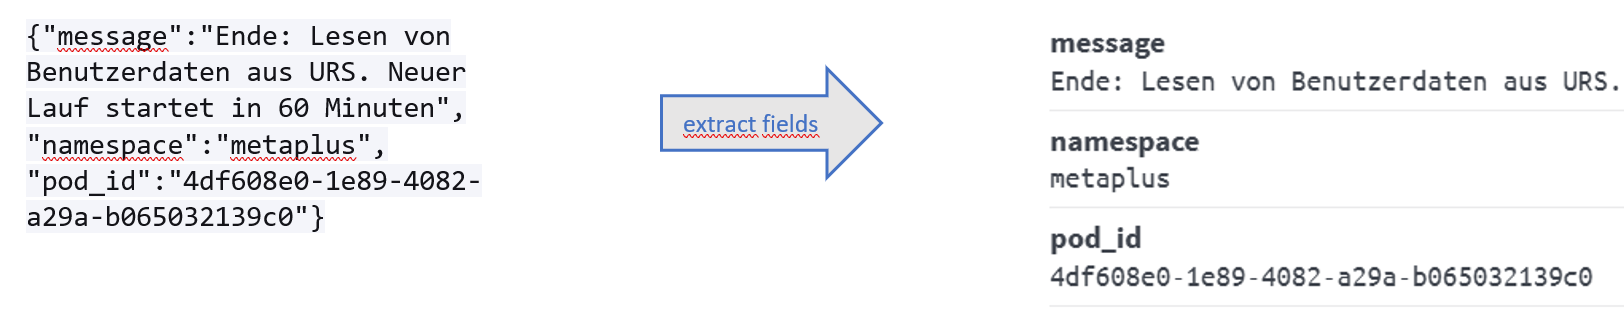
\includegraphics[scale=0.5]{img/10-appendix/input.png}
        \label{fig:input}
    \end{figure}
    
    How would you feel if you did have this feature?
    
    \begin{enumerate}
        \item I like it
        \item I expect it
        \item  I am neutral
        \item I can tolerate it
        \item I dislike it
    \end{enumerate}

    How would you feel if you did NOT have this feature?
    
    \begin{enumerate}
        \item I like it
        \item I expect it
        \item  I am neutral
        \item I can tolerate it
        \item I dislike it
    \end{enumerate}

    \clearpage
    \item \textbf{Sidebar with list of fields}

    Graylog displays all extracted fields in the sidebar list. In the example below the following fields were extracted: facility (string), full\_message (string),
    level (number), gl2\_processing\_timestamp (datetime), ... 
    
    Use Case: list of fields serves as a reference. You can filter logs using those fields.

    \begin{figure}[H]
        \centering
        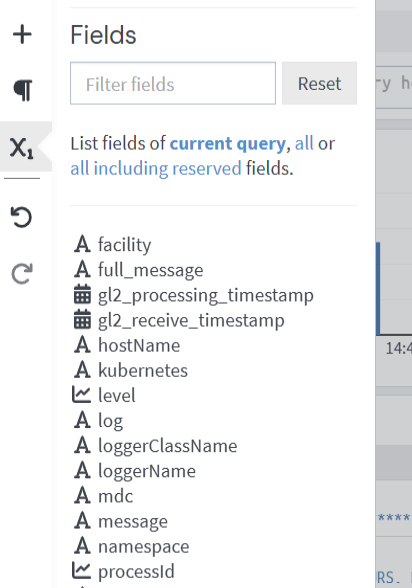
\includegraphics[scale=1]{img/10-appendix/fields.png}
        \label{fig:fields}
    \end{figure}

    How would you feel if you did have this feature?
    
    \begin{enumerate}
        \item I like it
        \item I expect it
        \item  I am neutral
        \item I can tolerate it
        \item I dislike it
    \end{enumerate}

    How would you feel if you did NOT have this feature?
    
    \begin{enumerate}
        \item I like it
        \item I expect it
        \item  I am neutral
        \item I can tolerate it
        \item I dislike it
    \end{enumerate}

    \clearpage
    \item \textbf{Add additional field with static value}

    Add an additional field with a static value to all incoming logs from a specific input. 
    
    Use Case: automatically append the field "cluster: test" to all incoming logs received from the test cluster.

    \begin{figure}[H]
        \centering
        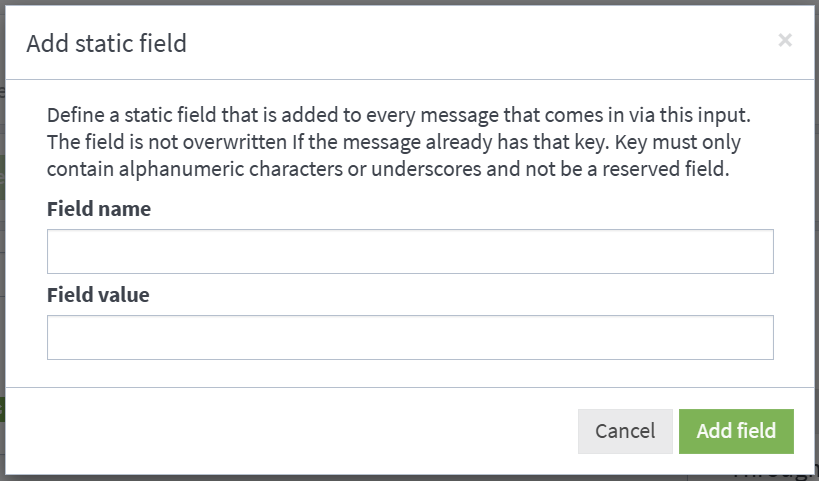
\includegraphics[scale=0.6]{img/10-appendix/static_field.png}
        \label{fig:static_field}
    \end{figure}

    How would you feel if you did have this feature?
    
    \begin{enumerate}
        \item I like it
        \item I expect it
        \item  I am neutral
        \item I can tolerate it
        \item I dislike it
    \end{enumerate}

    How would you feel if you did NOT have this feature?
    
    \begin{enumerate}
        \item I like it
        \item I expect it
        \item  I am neutral
        \item I can tolerate it
        \item I dislike it
    \end{enumerate}

    \clearpage
    \item \textbf{Search for Field Values}
    
    Search for messages with specific field values, e.g., search for messages where \textit{"namespace:cld AND level:1"}.

    \begin{figure}[H]
        \centering
        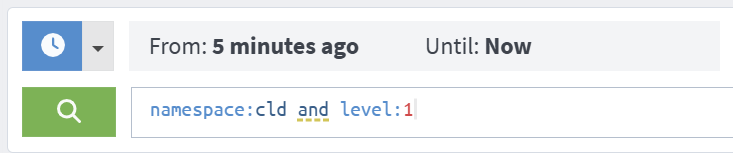
\includegraphics[]{img/10-appendix/search.png}
        \label{fig:search}
    \end{figure}

    How would you feel if you did have this feature?
    
    \begin{enumerate}
        \item I like it
        \item I expect it
        \item  I am neutral
        \item I can tolerate it
        \item I dislike it
    \end{enumerate}

    How would you feel if you did NOT have this feature?
    
    \begin{enumerate}
        \item I like it
        \item I expect it
        \item  I am neutral
        \item I can tolerate it
        \item I dislike it
    \end{enumerate}

    \clearpage
    \item \textbf{GROK Patterns}
    
    Graylog provides a customizable list of GROK patterns, which are predefined regular expression-based patterns which can be used to extract information such as email or IP-addresses, timestamps and many more. 
    
    Use Case: GROK Patterns for email.

    \begin{figure}[H]
        \centering
        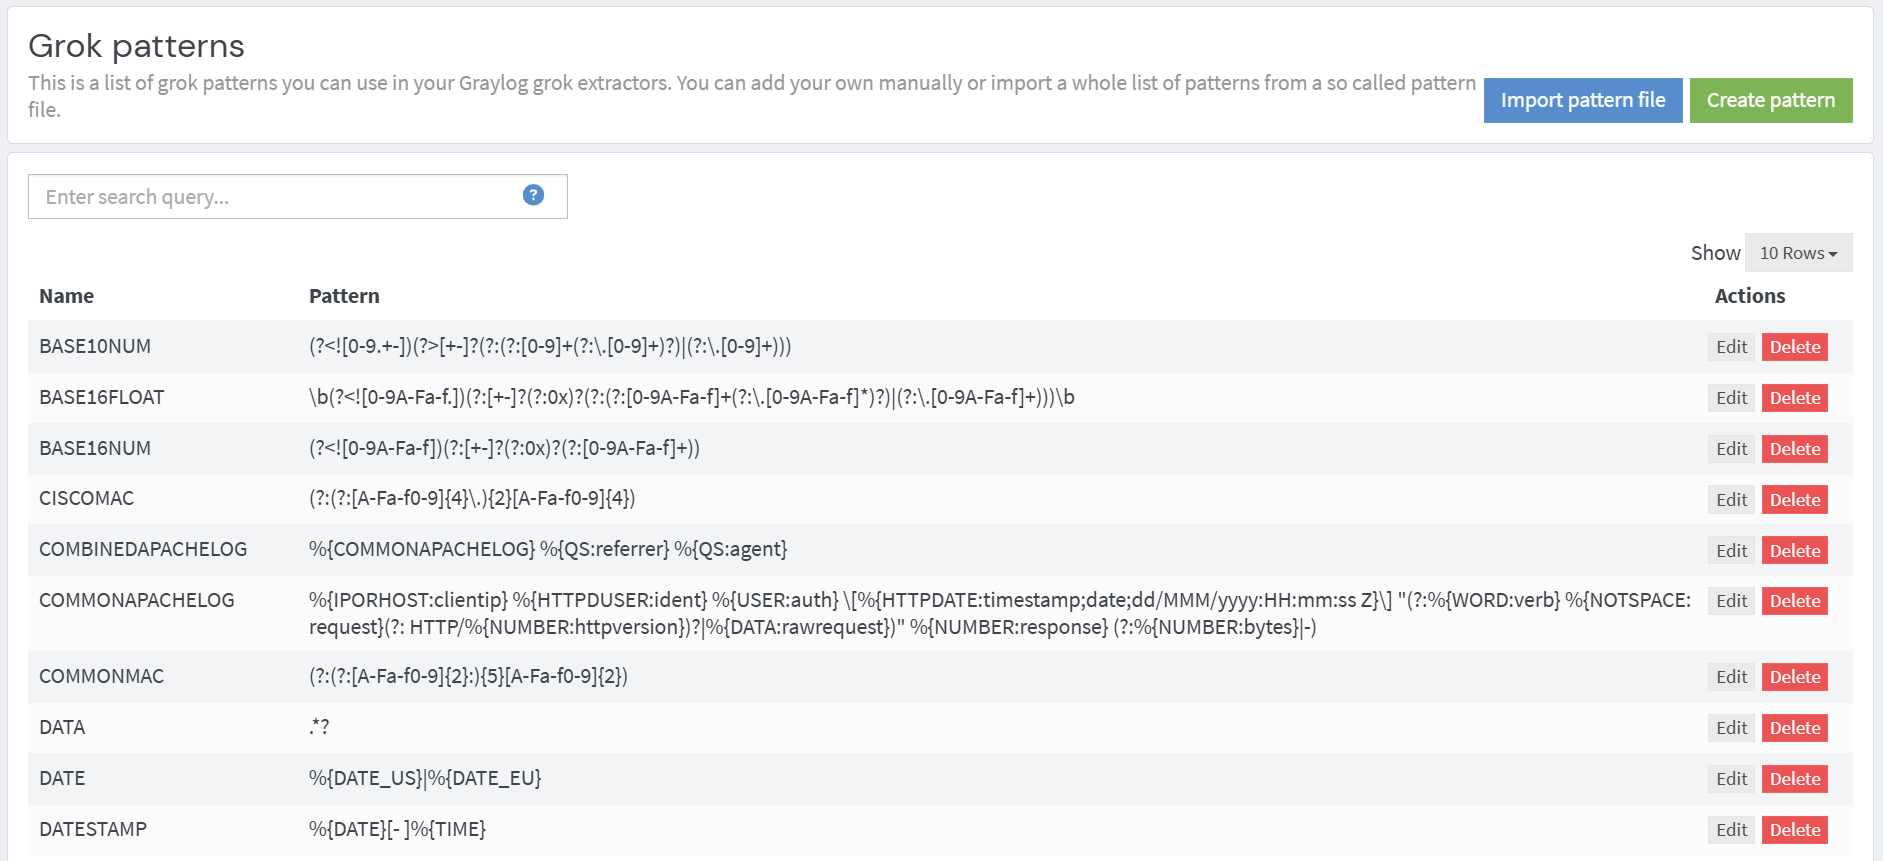
\includegraphics[scale=0.3]{img/10-appendix/grok.png}
        \label{fig:grok}
    \end{figure}

    How would you feel if you did have this feature?
    
    \begin{enumerate}
        \item I like it
        \item I expect it
        \item  I am neutral
        \item I can tolerate it
        \item I dislike it
    \end{enumerate}

    How would you feel if you did NOT have this feature?
    
    \begin{enumerate}
        \item I like it
        \item I expect it
        \item  I am neutral
        \item I can tolerate it
        \item I dislike it
    \end{enumerate}

    \clearpage
    \item \textbf{Save Search Queries}
    
    Save used search queries in a list with metadata: a title, description and summary. 
    
    Use Case: reuse effective search queries, allowing you and others to streamline the search process.

    \begin{figure}[H]
        \centering
        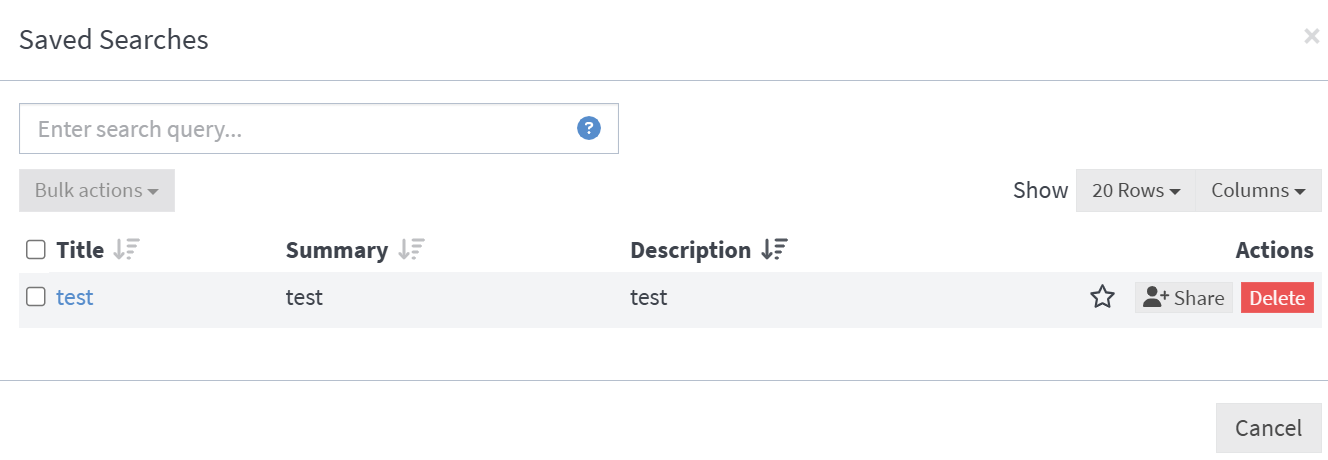
\includegraphics[scale=0.6]{img/10-appendix/description.png}
        \label{fig:description}
    \end{figure}

    How would you feel if you did have this feature?
    \begin{enumerate}
        \item I like it
        \item I expect it
        \item  I am neutral
        \item I can tolerate it
        \item I dislike it
    \end{enumerate}

    How would you feel if you did NOT have this feature?
    \begin{enumerate}
        \item I like it
        \item I expect it
        \item  I am neutral
        \item I can tolerate it
        \item I dislike it
    \end{enumerate}

    \clearpage
    \item\textbf{Export Search Queries to Dashboard as Widgets}
    
    Export saved searches into dashboard widgets.

    \begin{figure}[H]
        \centering
        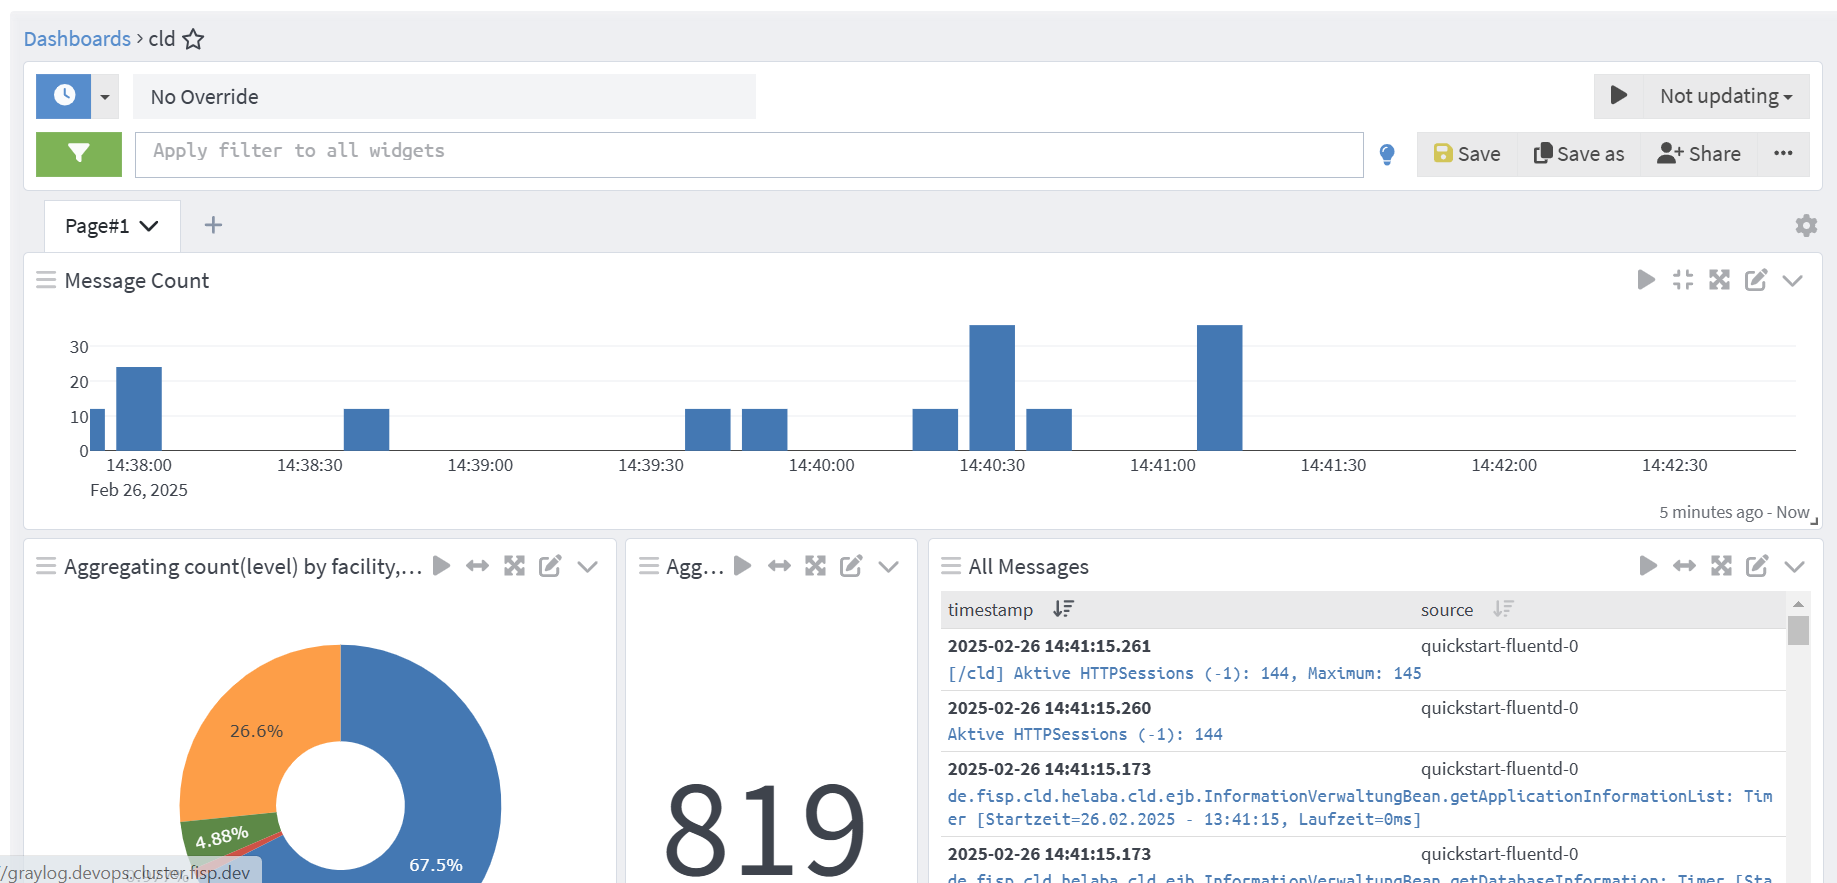
\includegraphics[scale=0.3]{img/10-appendix/dashboard.png}
        \label{fig:dashboard}
    \end{figure}

    How would you feel if you did have this feature?
    \begin{enumerate}
        \item I like it
        \item I expect it
        \item  I am neutral
        \item I can tolerate it
        \item I dislike it
    \end{enumerate}

    How would you feel if you did NOT have this feature?
    \begin{enumerate}
        \item I like it
        \item I expect it
        \item  I am neutral
        \item I can tolerate it
        \item I dislike it
    \end{enumerate}

    \clearpage
    \item \textbf{Custom Aggregations}
    
    Create aggregations (group by, metrics, sort) and visualize them (pie chart, graph, heat map etc.). 
    
    Use Case: group by field „level“ and count grouped values of all time.

    \begin{figure}[H]
        \centering
        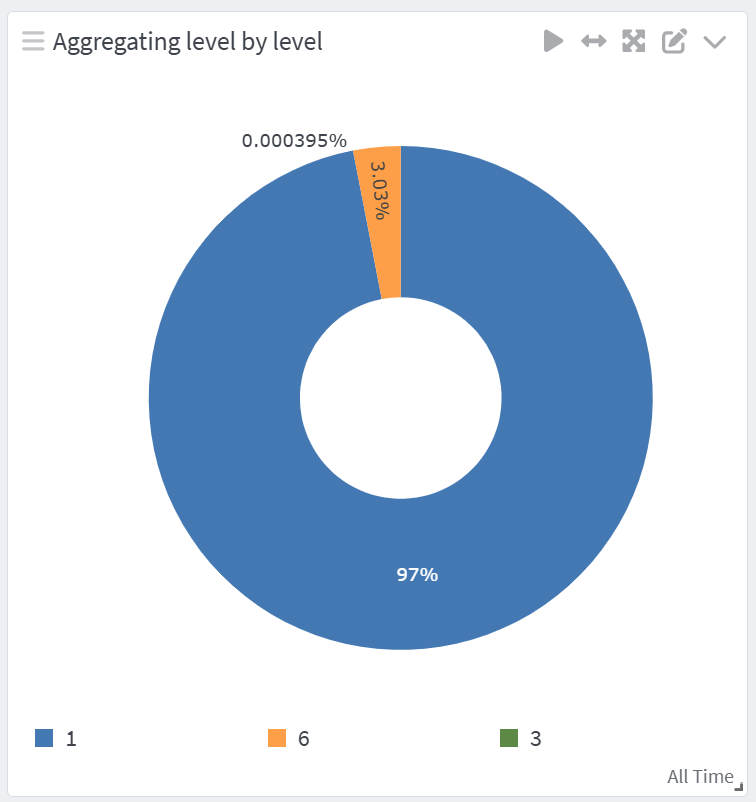
\includegraphics[scale=0.8]{img/10-appendix/level_count_all_time.png}
        \label{fig:level_count}
    \end{figure}

    How would you feel if you did have this feature?
    
    \begin{enumerate}
        \item I like it
        \item I expect it
        \item  I am neutral
        \item I can tolerate it
        \item I dislike it
    \end{enumerate}

    How would you feel if you did NOT have this feature?
    
    \begin{enumerate}
        \item I like it
        \item I expect it
        \item  I am neutral
        \item I can tolerate it
        \item I dislike it
    \end{enumerate}

    \clearpage
    \item \textbf{Real-Time Updates of Dashboards}
    
    Dashboards update automatically at scheduled intervals (e.g., every minute).

    \begin{figure}[H]
        \centering
        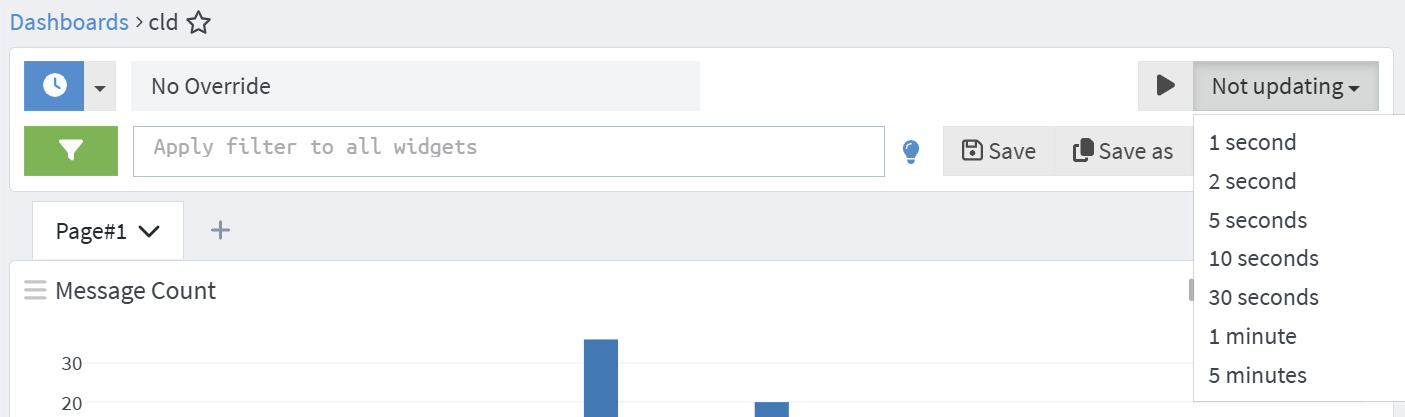
\includegraphics[scale=0.6]{img/10-appendix/dashboard_update.png}
        \label{fig:dashboard_update}
    \end{figure}

    How would you feel if you did have this feature?
    
    \begin{enumerate}
        \item I like it
        \item I expect it
        \item  I am neutral
        \item I can tolerate it
        \item I dislike it
    \end{enumerate}

    How would you feel if you did NOT have this feature?
    
    \begin{enumerate}
        \item I like it
        \item I expect it
        \item  I am neutral
        \item I can tolerate it
        \item I dislike it
    \end{enumerate}

    \clearpage
    \item \textbf{Search Time Range (Relative, Absolute)}
    
    Find logs within a specific time range by specifying exact timestamps or choosing a relative period (e.g., last 5 minutes, past 24 hours). 
    
    Use Case: set the time range to begin from the first occurrence of the failure.

    \begin{figure}[H]
        \centering
        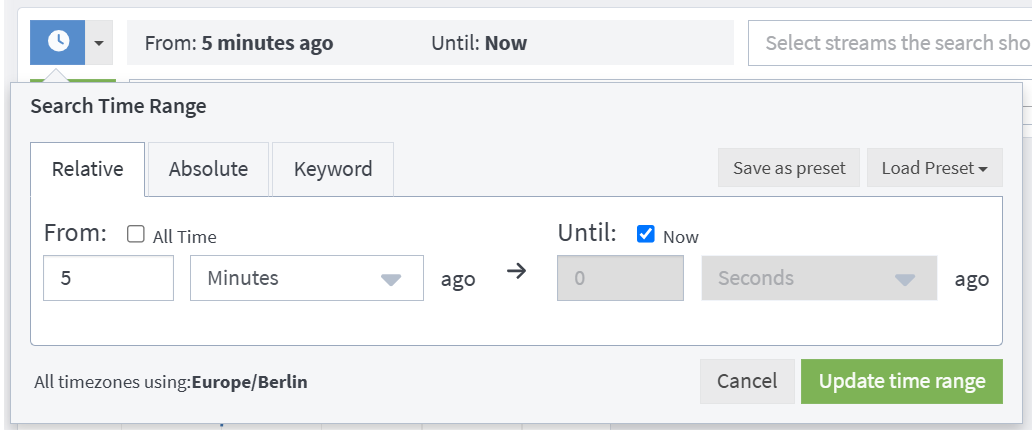
\includegraphics[scale=0.8]{img/10-appendix/timerange_relative.png}
        \label{fig:timerange_relative}
    \end{figure}

    How would you feel if you did have this feature?
    
    \begin{enumerate}
        \item I like it
        \item I expect it
        \item  I am neutral
        \item I can tolerate it
        \item I dislike it
    \end{enumerate}

    How would you feel if you did NOT have this feature?
    
    \begin{enumerate}
        \item I like it
        \item I expect it
        \item  I am neutral
        \item I can tolerate it
        \item I dislike it
    \end{enumerate}

    \clearpage
    \item \textbf{Search Time Range with Keywords}
    
    Use natural language keywords (e.g., "yesterday," "last hour") instead of manually setting time ranges. 
    
    Use Case: When a failure occurs and you know it happened within the last hour, use the keyword "last hour" to restrict the time range.

    \begin{figure}[H]
        \centering
        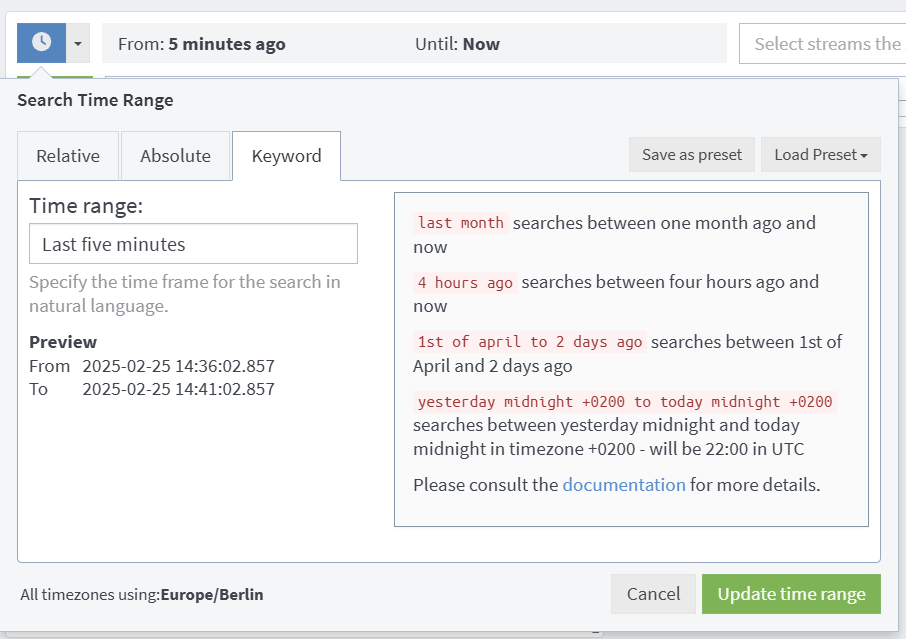
\includegraphics[scale=0.9]{img/10-appendix/timerange_keywords.png}
        \label{fig:timerange_keywords}
    \end{figure}

    How would you feel if you did have this feature?
    
    \begin{enumerate}
        \item I like it
        \item I expect it
        \item  I am neutral
        \item I can tolerate it
        \item I dislike it
    \end{enumerate}

    How would you feel if you did NOT have this feature?
    
    \begin{enumerate}
        \item I like it
        \item I expect it
        \item  I am neutral
        \item I can tolerate it
        \item I dislike it
    \end{enumerate}

    \clearpage
    \item \textbf{Show Surrounding Messages}
    
    View messages that occurred just before and after a selected log (e.g., 1 second to 1 minute). 
    
    Use Case: After identifying a relevant error log, narrow the log view to a 5-minute window before and after the message to gain better context.

    \begin{figure}[H]
        \centering
        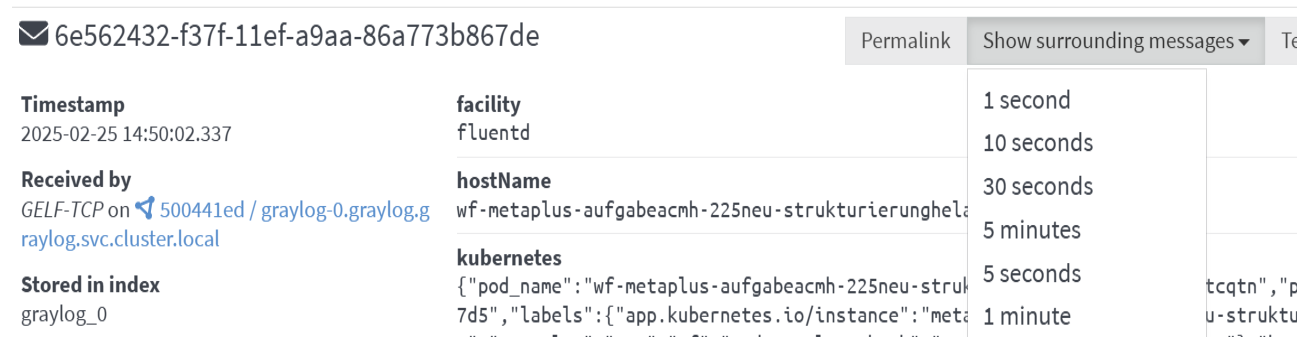
\includegraphics[scale=0.65]{img/10-appendix/surrounding_mes.png}
        \label{fig:surrounding_mes}
    \end{figure}

    How would you feel if you did have this feature?
    
    \begin{enumerate}
        \item I like it
        \item I expect it
        \item  I am neutral
        \item I can tolerate it
        \item I dislike it
    \end{enumerate}

    How would you feel if you did NOT have this feature?
    
    \begin{enumerate}
        \item I like it
        \item I expect it
        \item  I am neutral
        \item I can tolerate it
        \item I dislike it
    \end{enumerate}

    \clearpage
    \item \textbf{Highlighting}
    
    Field values can be highlighted in a certain color either by defining a rule or by selecting an existing field value to mark all its occurrences. 
    
    Use Case: highlight "INFO" with green, "WARN" with red. Highlight a specific process ID "X" with a distinct color to make it easily identifiable for monitoring.

    \begin{figure}[H]
        \centering
        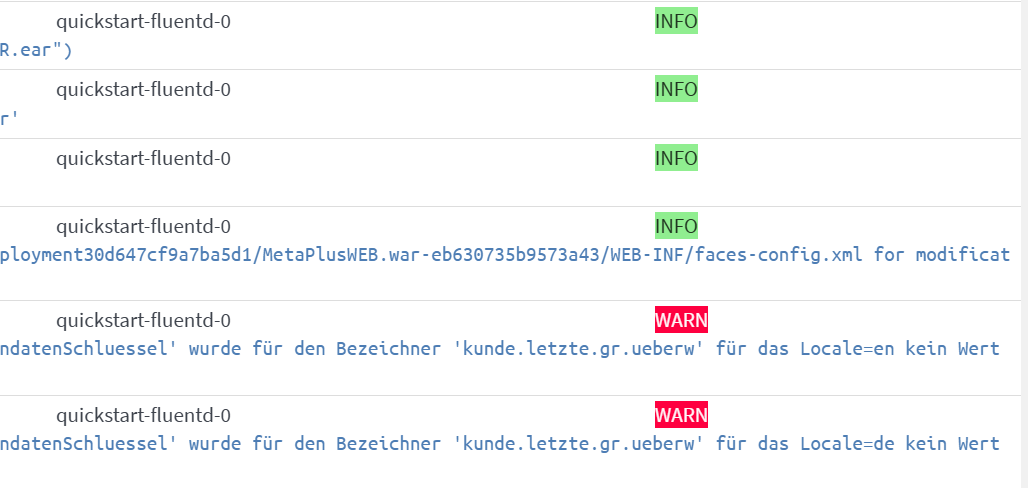
\includegraphics[scale=0.55]{img/10-appendix/highlight.png}
        \label{fig:highlight}
    \end{figure}

    How would you feel if you did have this feature?
    \begin{enumerate}
        \item I like it
        \item I expect it
        \item  I am neutral
        \item I can tolerate it
        \item I dislike it
    \end{enumerate}

    How would you feel if you did NOT have this feature?
    \begin{enumerate}
        \item I like it
        \item I expect it
        \item  I am neutral
        \item I can tolerate it
        \item I dislike it
    \end{enumerate}

    \clearpage
    \item \textbf{Alerts (Events, Notifications)}
    
    Notifications are sent (via email, Teams, or Slack) when an event occurs. In Graylog, this feature is known as "alerts."

    \begin{figure}[H]
        \centering
        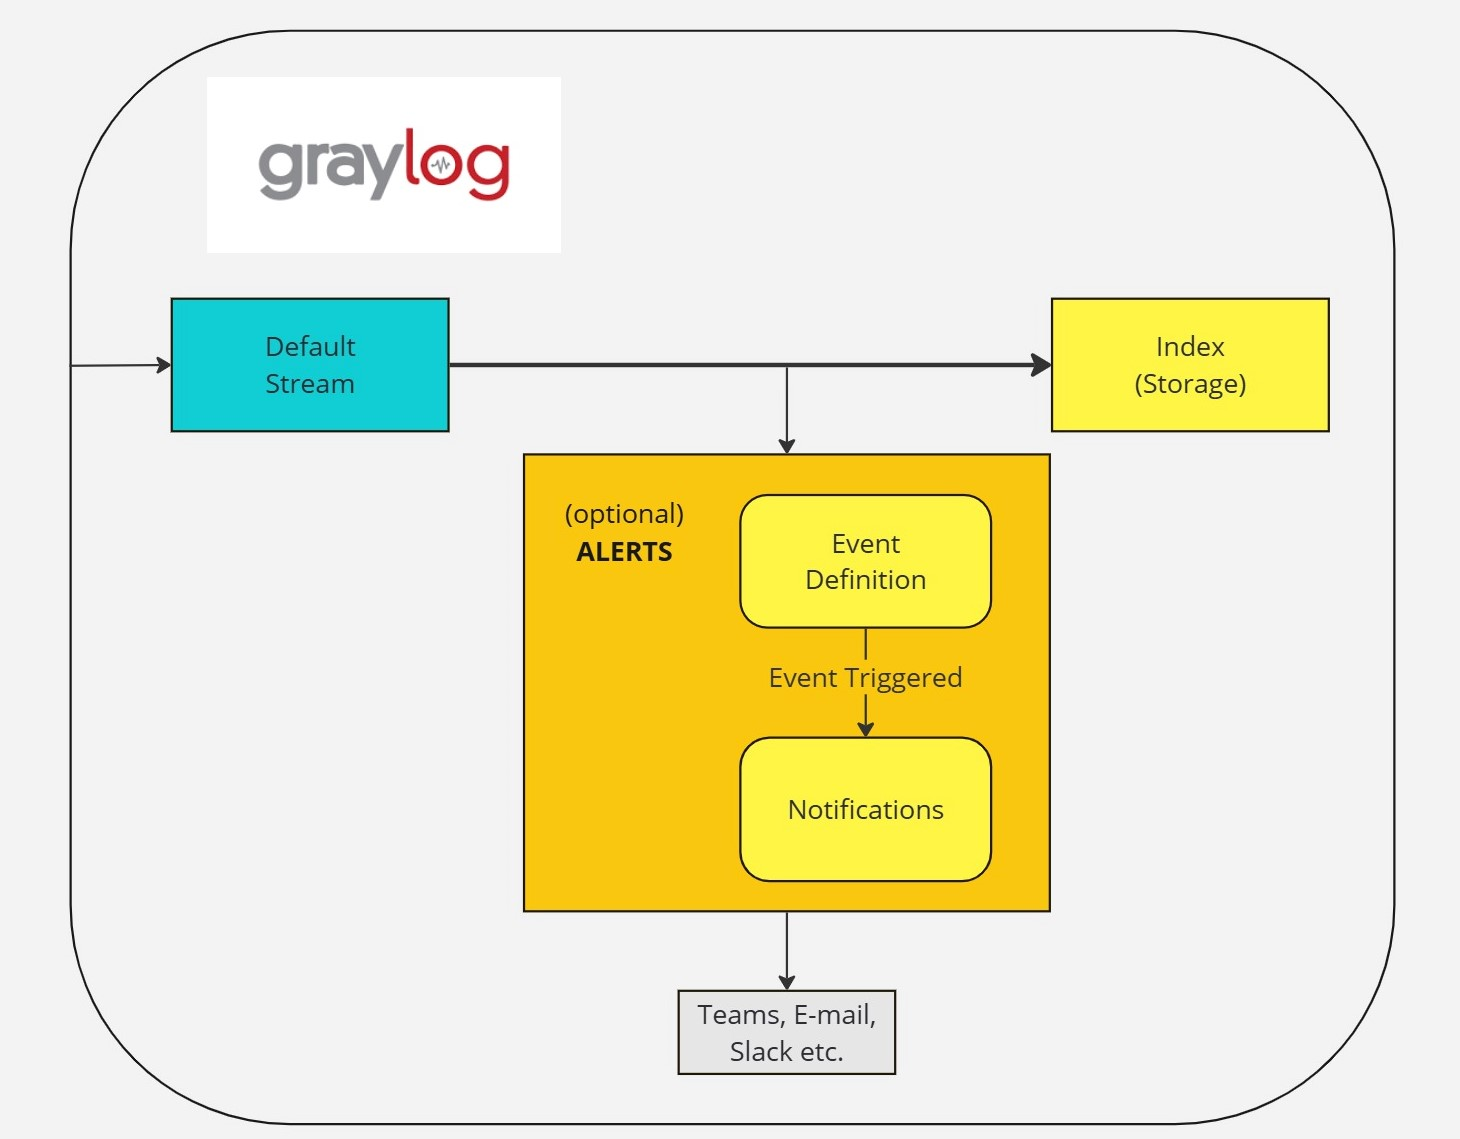
\includegraphics[scale=0.35]{img/10-appendix/alerts.jpg}
        \label{fig:alerts}
    \end{figure}

    How would you feel if you did have this feature?
    \begin{enumerate}
        \item I like it
        \item I expect it
        \item  I am neutral
        \item I can tolerate it
        \item I dislike it
    \end{enumerate}

    How would you feel if you did NOT have this feature?
    \begin{enumerate}
        \item I like it
        \item I expect it
        \item  I am neutral
        \item I can tolerate it
        \item I dislike it
    \end{enumerate}

    \clearpage
    \item \textbf{Stream Rules}
    
    Incoming logs can be sorted into different streams based on custom rules; otherwise, they are routed to the default stream. 
    
    Use Case: Sort logs from different microservices into separate streams while retaining all messages in the default stream for a complete overview. If field "namespace=cld" is true route to Stream 1, else route to default stream.

    \begin{figure}[H]
        \centering
        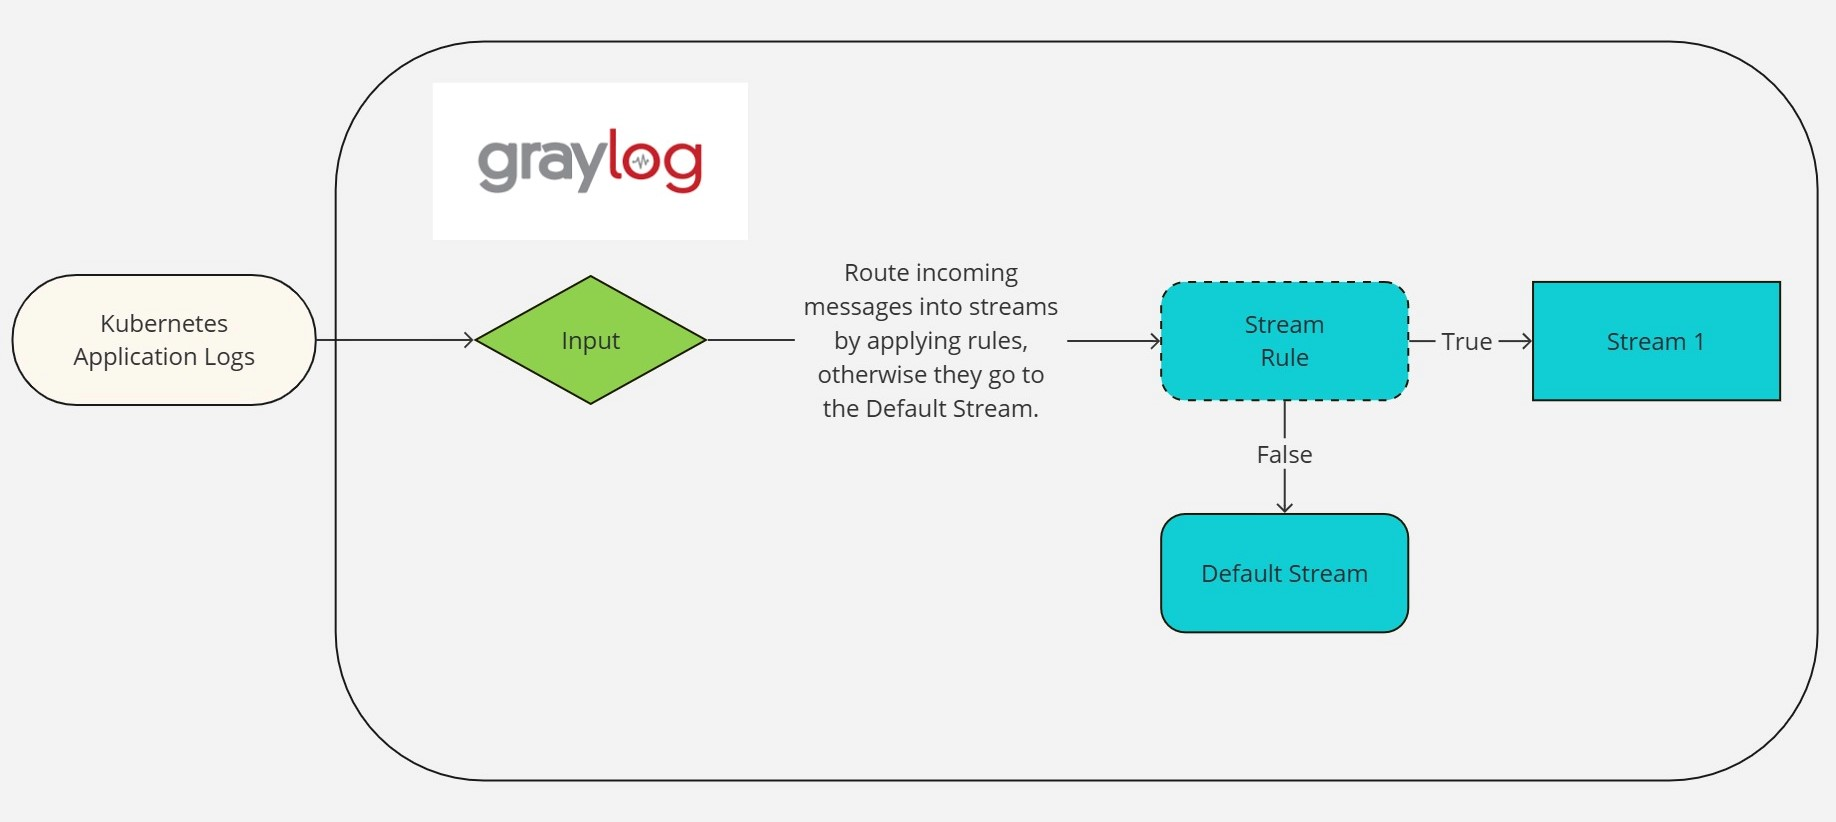
\includegraphics[scale=0.3]{img/10-appendix/streams.jpg}
        \label{fig:streams}
    \end{figure}

    How would you feel if you did have this feature?
    \begin{enumerate}
        \item I like it
        \item I expect it
        \item  I am neutral
        \item I can tolerate it
        \item I dislike it
    \end{enumerate}

    How would you feel if you did NOT have this feature?
    \begin{enumerate}
        \item I like it
        \item I expect it
        \item  I am neutral
        \item I can tolerate it
        \item I dislike it
    \end{enumerate}

    \clearpage
    \item \textbf{Pipeline Processing}
    
    Create a pipeline consisting of multiple stages, each applying specific rules and actions to process stream messages. 
    
    Use Case: Extract specific values, e.g., user name, using a pipeline stage before the log is stored.

    \begin{figure}[H]
        \centering
        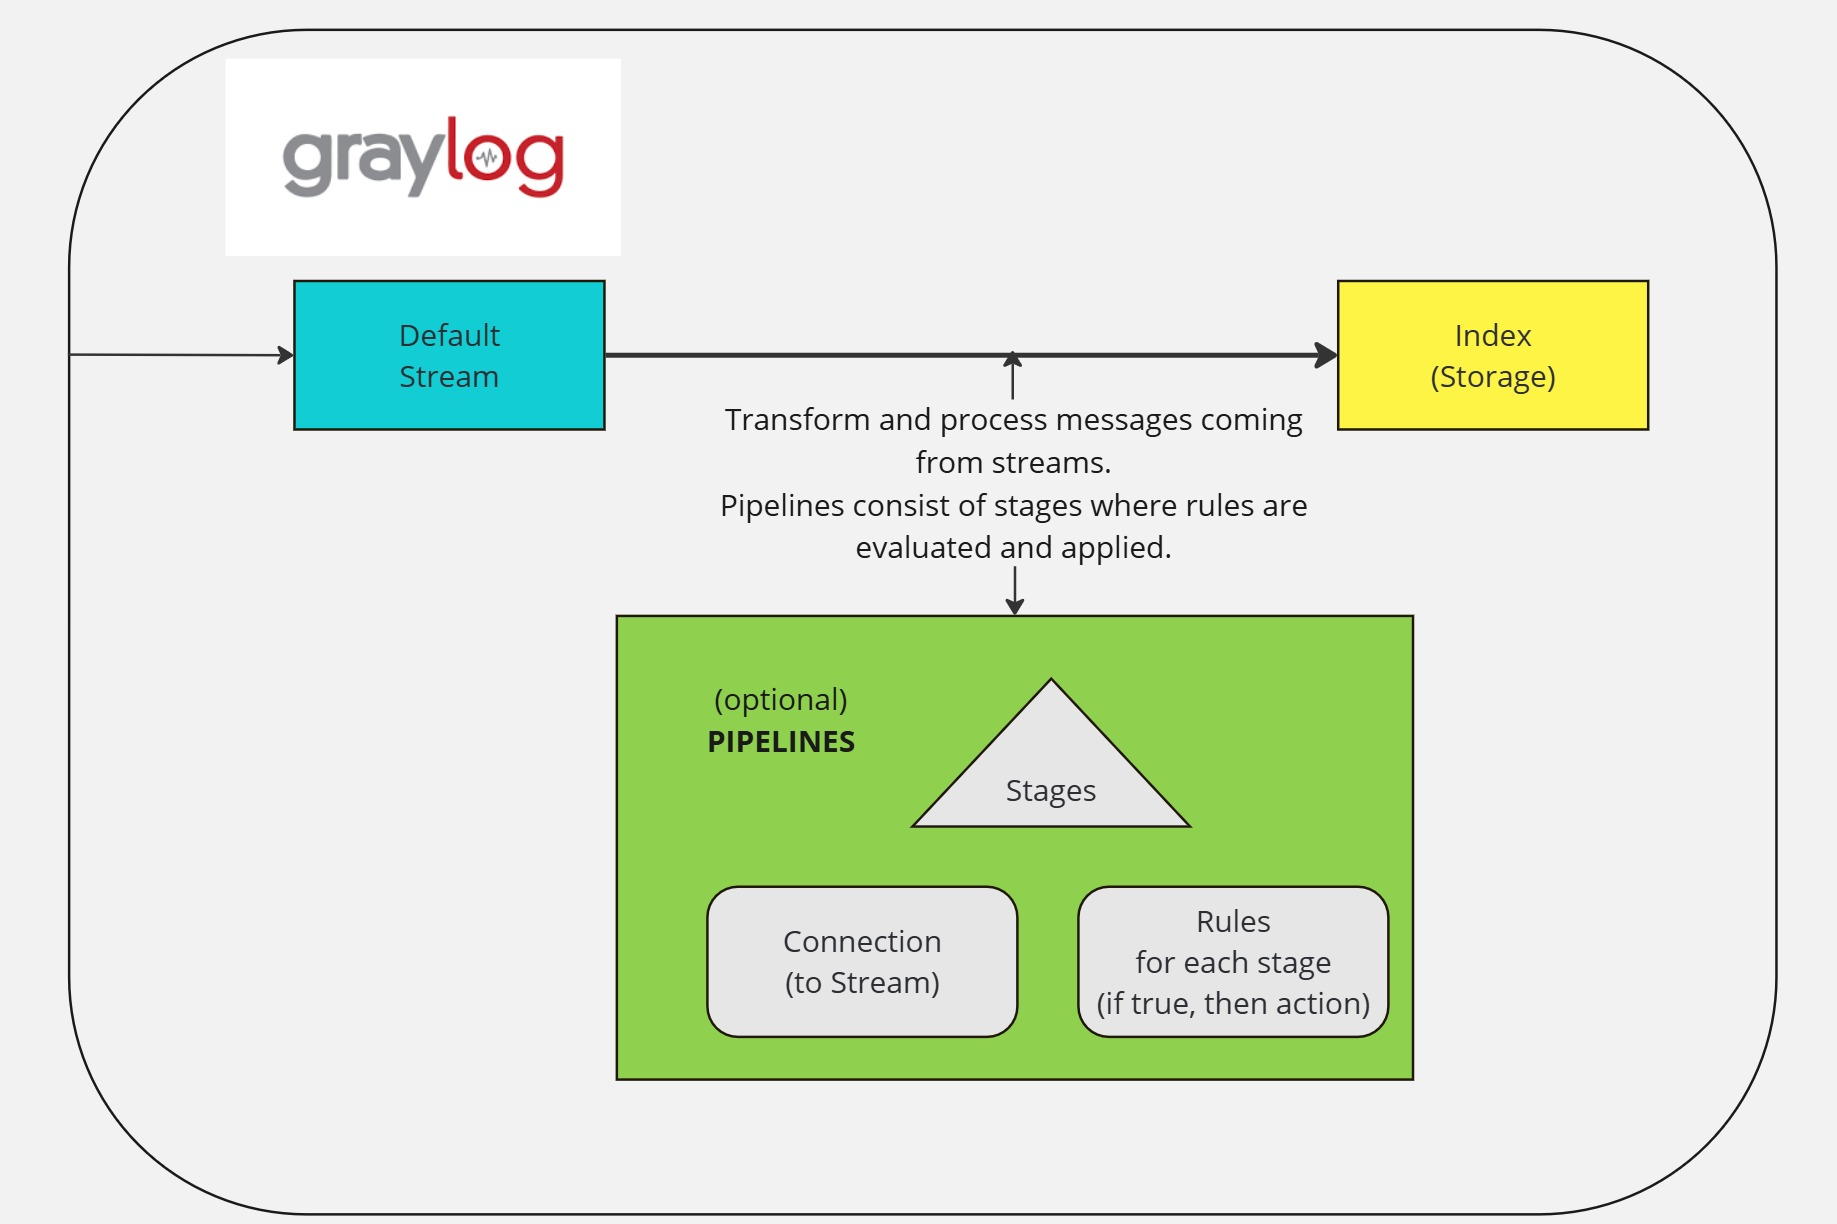
\includegraphics[scale=0.23]{img/10-appendix/pipelines.jpg}
        \label{fig:pipelines}
    \end{figure}

    How would you feel if you did have this feature?
    \begin{enumerate}
        \item I like it
        \item I expect it
        \item  I am neutral
        \item I can tolerate it
        \item I dislike it
    \end{enumerate}

    How would you feel if you did NOT have this feature?
    \begin{enumerate}
        \item I like it
        \item I expect it
        \item  I am neutral
        \item I can tolerate it
        \item I dislike it
    \end{enumerate}

    \clearpage
    \item \textbf{Lookup Tables}
    
    Lookup Tables can be used to retrieve data from external sources (e.g., API calls, CSV files) and enrich messages with additional fields. 
    
    Use Case: message contains field "userID" with value "6". Look up this value in a lookup table and write the result into a new field => userName="John Doe".

    \begin{figure}[H]
        \centering
        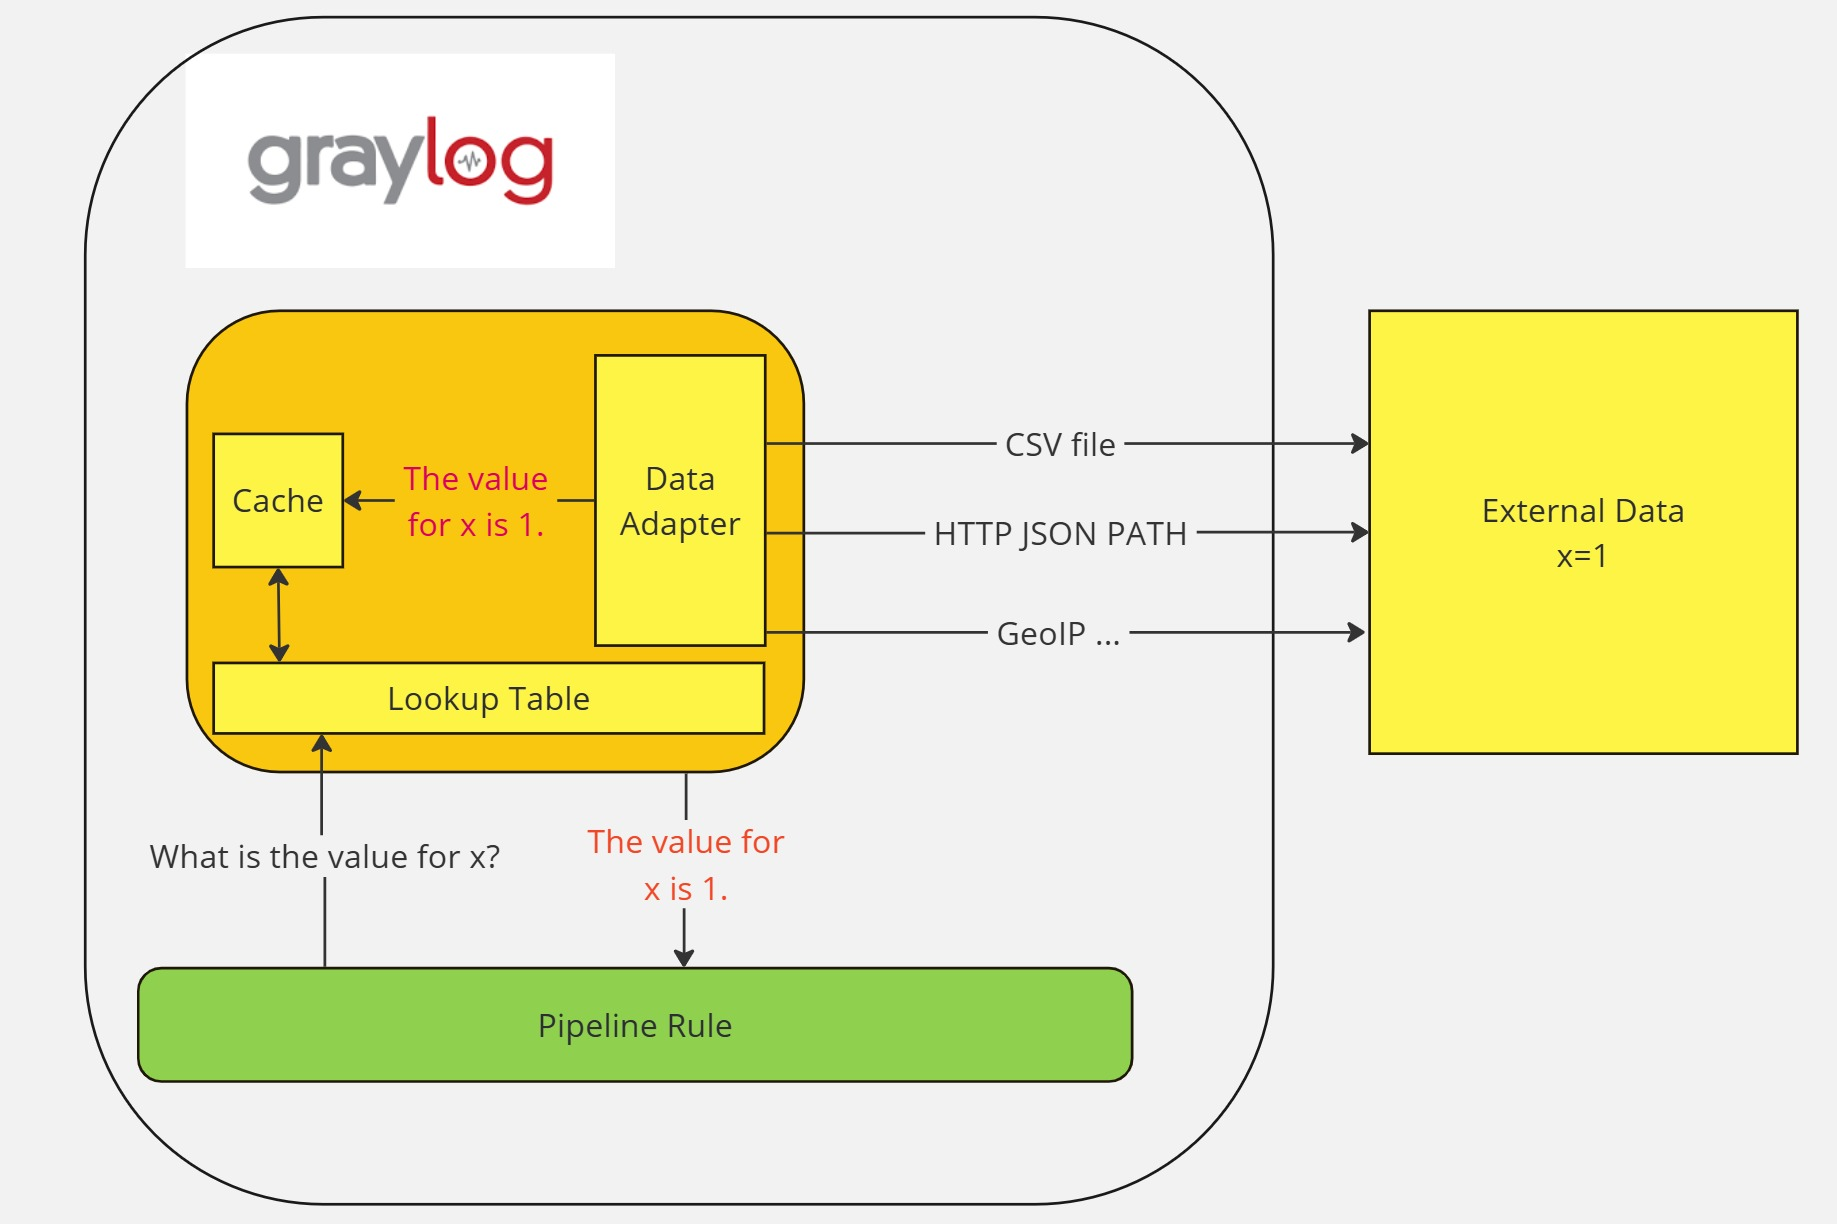
\includegraphics[scale=0.23]{img/10-appendix/lookup_table.jpg}
        \label{fig:lookup_table}
    \end{figure}

    How would you feel if you did have this feature?
    \begin{enumerate}
        \item I like it
        \item I expect it
        \item  I am neutral
        \item I can tolerate it
        \item I dislike it
    \end{enumerate}

    How would you feel if you did NOT have this feature?
    \begin{enumerate}
        \item I like it
        \item I expect it
        \item  I am neutral
        \item I can tolerate it
        \item I dislike it
    \end{enumerate}

    \clearpage
    \item \textbf{Decorators}
    
    Decorators modify message field information in real time without altering the actual data. Applied at the stream level, they adjust how messages appear in searches without persisting changes. Examples include using pipelines or lookup tables as decorators.

    \begin{figure}[H]
        \centering
        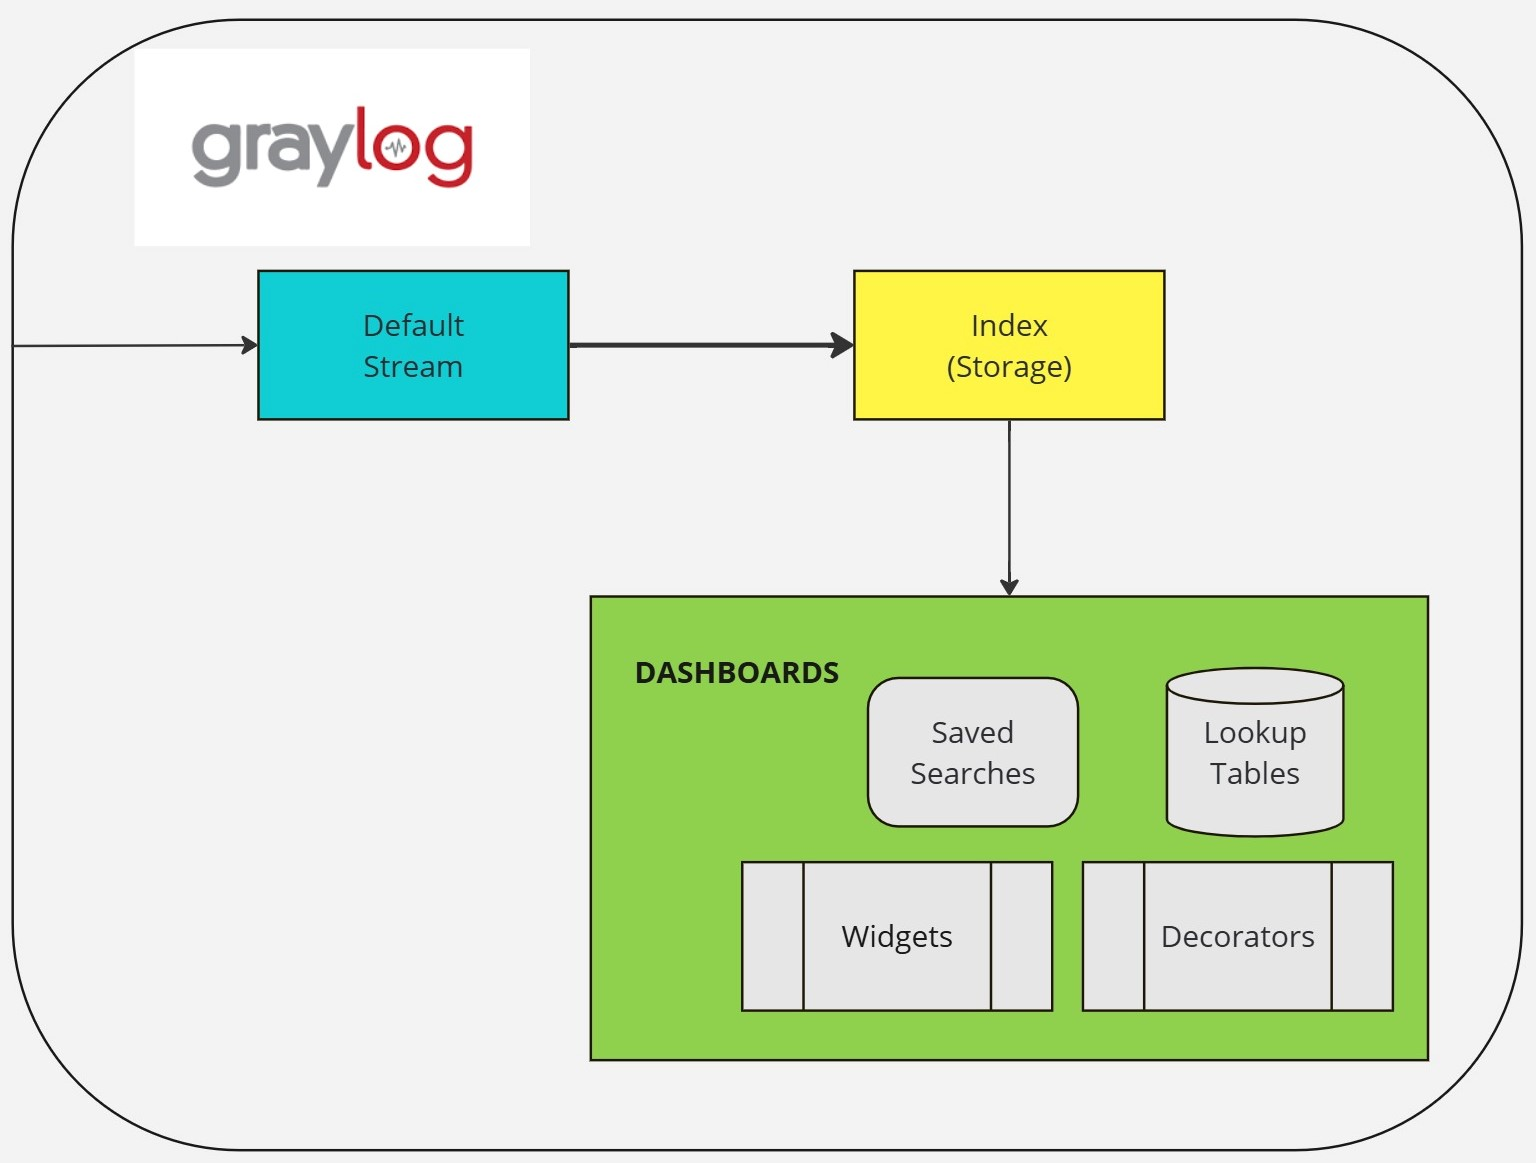
\includegraphics[scale=0.3]{img/10-appendix/dashboards.jpg}
        \label{fig:dashboards}
    \end{figure}

    How would you feel if you did have this feature?
    \begin{enumerate}
        \item I like it
        \item I expect it
        \item  I am neutral
        \item I can tolerate it
        \item I dislike it
    \end{enumerate}

    How would you feel if you did NOT have this feature?
    \begin{enumerate}
        \item I like it
        \item I expect it
        \item  I am neutral
        \item I can tolerate it
        \item I dislike it
    \end{enumerate}

    \clearpage
    \item \textbf{Export as CSV}
    
    A subset of the currently queried fields can be downloaded as a CSV file. 
    
    Use Case: download filtered logs to share with the client.

    How would you feel if you did have this feature?
    \begin{enumerate}
        \item I like it
        \item I expect it
        \item  I am neutral
        \item I can tolerate it
        \item I dislike it
    \end{enumerate}

    How would you feel if you did NOT have this feature?
    \begin{enumerate}
        \item I like it
        \item I expect it
        \item  I am neutral
        \item I can tolerate it
        \item I dislike it
    \end{enumerate}

    \clearpage
    \item \textbf{Customizable Index Sets}
    
    A Graylog stream write messages to index sets. Create and configure indices to manage how and where stream logs are stored. You could, for example, have different retention times for certain streams. 
    
    Use Case: Retain logs for only 1 day in the test environment, while keeping production logs for 30 days.

    \begin{figure}[H]
        \centering
        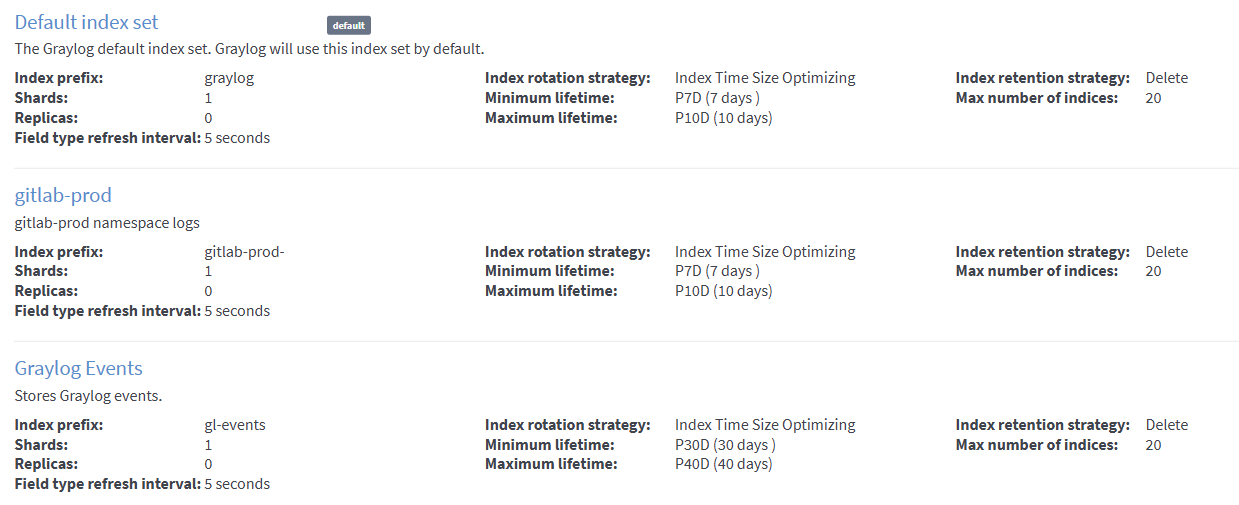
\includegraphics[scale=0.68]{img/10-appendix/indices.png}
        \label{fig:indices}
    \end{figure}

    How would you feel if you did have this feature?
    \begin{enumerate}
        \item I like it
        \item I expect it
        \item  I am neutral
        \item I can tolerate it
        \item I dislike it
    \end{enumerate}

    How would you feel if you did NOT have this feature?
    \begin{enumerate}
        \item I like it
        \item I expect it
        \item  I am neutral
        \item I can tolerate it
        \item I dislike it
    \end{enumerate}

    \clearpage
    \item \textbf{Sidecars}
    
    Graylog Sidecar is a lightweight configuration management system for log collectors. It provides a framework for managing log collectors, such as Winlogbeat, Filebeat, and NXLog. 
    
    Use Case: Deploy a Graylog sidecar on the server to collect logs if an application is not yet running on the Kubernetes cluster.

    \begin{figure}[H]
        \centering
        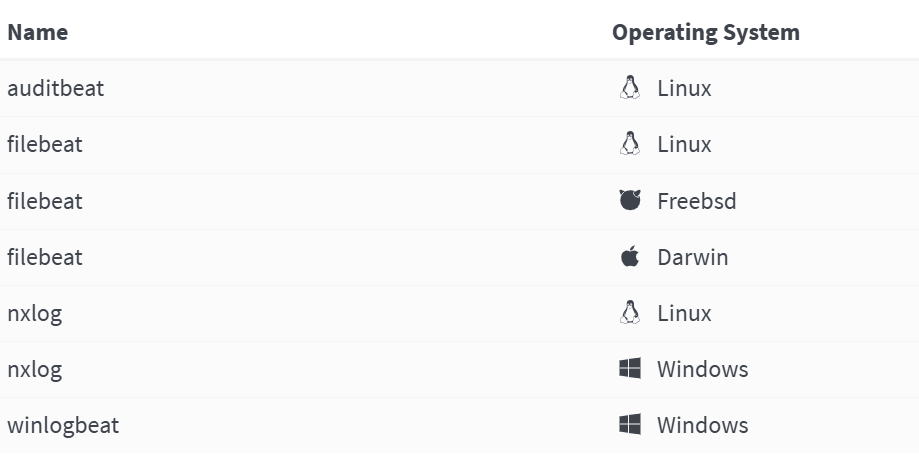
\includegraphics[scale=0.8]{img/10-appendix/sidecar_collectors.png}
        \label{fig:sidecar_collectors}
    \end{figure}

    How would you feel if you did have this feature?
    \begin{enumerate}
        \item I like it
        \item I expect it
        \item  I am neutral
        \item I can tolerate it
        \item I dislike it
    \end{enumerate}

    How would you feel if you did NOT have this feature?
    \begin{enumerate}
        \item I like it
        \item I expect it
        \item  I am neutral
        \item I can tolerate it
        \item I dislike it
    \end{enumerate}

    \clearpage
    \item \textbf{Content Packs (Pre-Built Setups)}
    
    Use pre-built configurations (by Graylog or user-built) for faster setup. 
    
    Use Case: Share pre-built configurations, such as dashboards and pipelines, with other Graylog instances to reduce work for other teams.

    \begin{figure}[H]
        \centering
        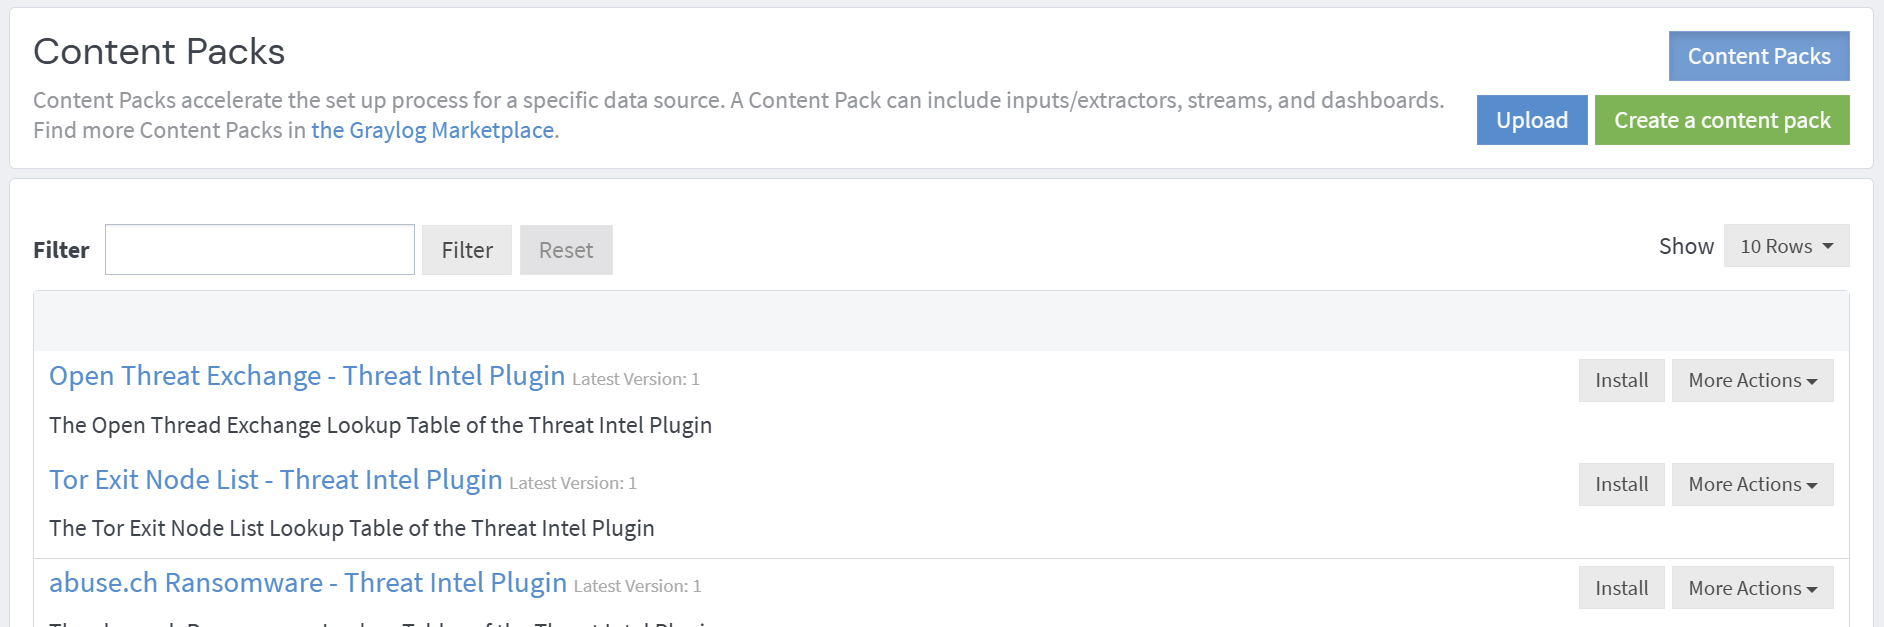
\includegraphics[scale=0.3]{img/10-appendix/content_packs.png}
        \label{fig:content_packs}
    \end{figure}

    How would you feel if you did have this feature?
    \begin{enumerate}
        \item I like it
        \item I expect it
        \item  I am neutral
        \item I can tolerate it
        \item I dislike it
    \end{enumerate}

    How would you feel if you did NOT have this feature?
    \begin{enumerate}
        \item I like it
        \item I expect it
        \item  I am neutral
        \item I can tolerate it
        \item I dislike it
    \end{enumerate}

    \clearpage
    \item \textbf{Authentication Service}
        
    Integrate with Active Directory (AD) or LDAP for user authentication and access management. 
    
    Use Case: All internal company users can immediately access and start using Graylog without additional setup.

    \begin{figure}[H]
        \centering
        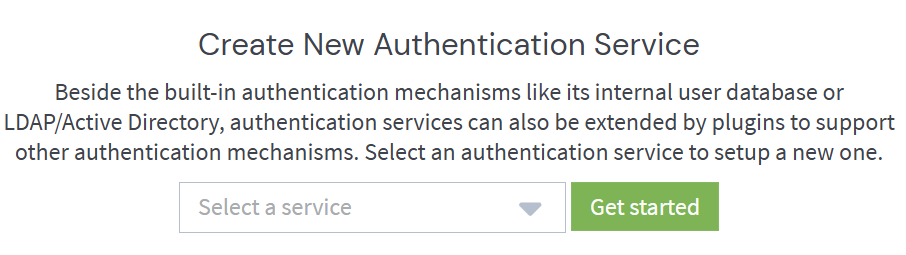
\includegraphics[scale=0.6]{img/10-appendix/authentication.png}
        \label{fig:authentication}
    \end{figure}

    How would you feel if you did have this feature?
    \begin{enumerate}
        \item I like it
        \item I expect it
        \item  I am neutral
        \item I can tolerate it
        \item I dislike it
    \end{enumerate}

    How would you feel if you did NOT have this feature?
    \begin{enumerate}
        \item I like it
        \item I expect it
        \item  I am neutral
        \item I can tolerate it
        \item I dislike it
    \end{enumerate}

    \clearpage
    \item \textbf{Roles}
    
    Use pre-built roles with permission levels to control access to features and data. A user can be assigned multiple roles. 
    
    Use Case: The owner of a stream can share logs with team colleagues by assigning them roles such as Viewer or Manager. Other users, except admins, cannot see the stream.

    \begin{figure}[H]
        \centering
        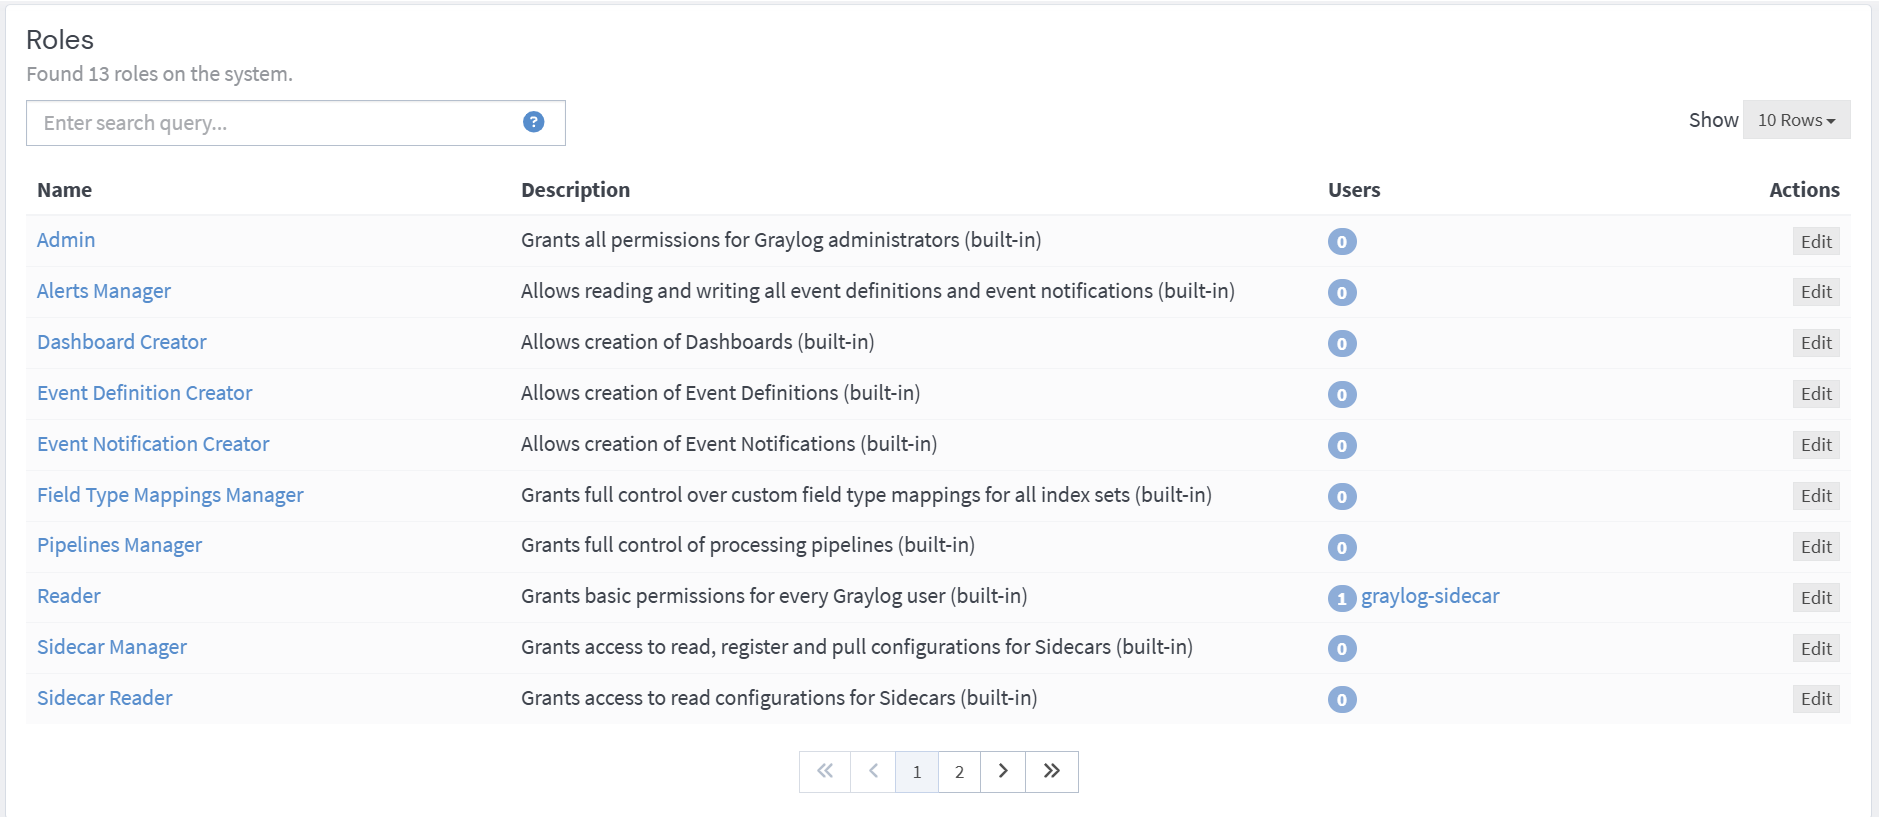
\includegraphics[scale=0.3]{img/10-appendix/roles.png}
        \label{fig:roles}
    \end{figure}

    How would you feel if you did have this feature?
    \begin{enumerate}
        \item I like it
        \item I expect it
        \item  I am neutral
        \item I can tolerate it
        \item I dislike it
    \end{enumerate}

    How would you feel if you did NOT have this feature?
    \begin{enumerate}
        \item I like it
        \item I expect it
        \item  I am neutral
        \item I can tolerate it
        \item I dislike it
    \end{enumerate}
    
\end{enumerate}

\end{document}